% Problems, Chapter 16: Radiation Damping, Classical Models of Charged Particles
% Jackson, Classical Electrodynamics, 3rd ed.
% Requires: amsmath, amssymb, tikz

\section*{Problems}

\Needspace{5\baselineskip}
\par\bigskip
\noindent\textbf{16.1}\quad A nonrelativistic particle of charge $e$ and mass $m$ is bound by a linear, isotropic, restoring force with force constant $m\omega_{0}^{2}$.

Using (16.13) and (16.16) of Section 16.2, show that the energy and angular momentum of the particle both decrease exponentially from their initial values as $e^{-\Gamma t}$, where $\Gamma=\omega_{0}^{2}\tau$. Quantum mechanically, the mean excitation energy of an oscillator decays in exactly the same way because the total radiative transition probability for a state with quantum numbers $n_{0}$, $l_{0}$ is $\Gamma(n_{0},l_{0})=n_{0}\Gamma$. The decay of the angular momentum approaches the classical law only for $l_{0}\gg1$.
\solution

We use Gaussian units and write $\tau_r=2e^2/(3mc^3)$ for the
radiation-reaction time (the $\tau$ of this question). The equations
(16.13) and (16.16) describe \emph{secular}, orbit-averaged changes;
they require $\omega_0\tau_r\ll1$.
For $V=\tfrac12m\omega_0^2r^2$, their explicit forms are
\[
\frac{d\mathcal E}{dt}=-\frac{\tau_r}{m}
\left\langle(V')^2\right\rangle
=-m\tau_r\omega_0^4\langle r^2\rangle,
\qquad
\frac{d\mathbf L}{dt}=-\frac{\tau_r}{m}
\left\langle\frac{V'}r\right\rangle\mathbf L
=-\tau_r\omega_0^2\mathbf L.
\]
To express the first in terms of energy, write the unperturbed orbit
$\mathbf r=\mathbf A\cos\omega_0t+\mathbf B\sin\omega_0t$.
A full-period average gives
\[
\langle r^2\rangle=\frac{A^2+B^2}{2},\quad
\langle v^2\rangle=\omega_0^2\frac{A^2+B^2}{2},\quad
\mathcal E=\frac m2\langle v^2+\omega_0^2r^2\rangle
=m\omega_0^2\langle r^2\rangle.
\]
Thus both differential equations have the same decay constant:
\[
\boxed{\mathcal E(t)=\mathcal E(0)e^{-\Gamma t},\qquad
\mathbf L(t)=\mathbf L(0)e^{-\Gamma t},\qquad
\Gamma=\omega_0^2\tau_r.}
\]
The angular-momentum direction is unchanged. The energy here is the
slowly varying orbital energy; small within-cycle corrections are
outside the averaging approximation. In the reduced-order oscillator
$\ddot{\mathbf r}+\Gamma\dot{\mathbf r}+\omega_0^2\mathbf r=0$,
the coordinate amplitude decays as $e^{-\Gamma t/2}$, giving the same
energy envelope. The quantum comparison in the question concerns
excitation energy above the ground state, whose zero-point energy is
not radiated away.

\Needspace{5\baselineskip}
\par\bigskip
\noindent\textbf{16.2}\quad A nonrelativistic electron of charge $-e$ and mass $m$ bound in an attractive Coulomb potential ($-Ze^{2}/r$) moves in a circular orbit in the absence of radiation reaction.
\begin{enumerate}
\item[(a)] Show that both the energy and angular-momentum equations (16.13) and (16.16) lead to the solution for the slowly changing orbit radius,
\[
r^{3}(t)=r_{0}^{3}-9Z(c\tau)^{3}\frac{t}{\tau}
\]
where $r_{0}$ is the value of $r(t)$ at $t=0$.
\item[(b)] For circular orbits in a Bohr atom the orbit radius and the principal quantum number $n$ are related by $r=n^{2}a_{0}/Z$. If the transition probability for transitions from $n\to(n-1)$ is defined as $-dn/dt$, show that the result of part a agrees with that found in Problem 14.21.
\item[(c)] From part a calculate the numerical value of the times taken for a mu meson of mass $m=207m_{e}$ to fall from a circular orbit with principal quantum number $n_{1}=10$ to one with $n_{2}=4$, and $n_{2}=1$. These are reasonable estimates of the time taken for a mu meson to cascade down to its lowest orbit after capture by an isolated atom.
\end{enumerate}
\solution

Put $A=Ze^2$ and $\tau_r=2e^2/(3mc^3)$. The orbit remains nearly
circular when its radiative evolution is slow compared with a period.

\textbf{(a)} Circular force balance and the orbital energy give
\[
v^2=\frac A{mr},\qquad
\mathcal E=-\frac A{2r},\qquad
L=\sqrt{mAr}.
\]
The energy equation is
\[
\frac A{2r^2}\dot r
=-\frac{\tau_r}{m}\frac{A^2}{r^4},
\quad\hbox{hence}\quad
\dot r=-\frac{2\tau_r A}{mr^2}.
\]
Independently, the angular-momentum equation gives
\[
\dot L=-\frac{\tau_r A}{mr^3}L,
\qquad \dot L=\frac L{2r}\dot r,
\]
which yields the same $\dot r$. Multiply it by $3r^2$ and use
$e^2/m=3c^3\tau_r/2$:
\[
\frac{d(r^3)}{dt}=-\frac{6\tau_r Ze^2}{m}
=-9Zc^3\tau_r^2.
\]
Integration from $t=0$ gives
\[
\boxed{r^3(t)=r_0^3-9Z(c\tau_r)^3\frac t{\tau_r}.}
\]
This formal shrinking-orbit law ceases to apply when the orbit is no
longer nonrelativistic and slowly varying; it does not describe the
final singular collapse of a point-particle model reliably.

\textbf{(b)} For a particle of mass $m$, define its Bohr length
$a_m=\hbar^2/(me^2)$, so $r=n^2a_m/Z$.
Since $r^3=n^6a_m^3/Z^3$, differentiation gives
\[
6n^5\frac{a_m^3}{Z^3}\dot n=-9Zc^3\tau_r^2,
\qquad
-\dot n=\frac{3Z^4c^3\tau_r^2}{2a_m^3n^5}.
\]
Substitute $a_m=\hbar/(mc\alpha)$ and
$\tau_r=2\alpha\hbar/(3mc^2)$:
\[
\boxed{-\dot n=\frac23\alpha(Z\alpha)^4
\frac{mc^2}{\hbar}\frac1{n^5},}
\]
exactly the classical transition-rate estimate in 14.21.

\textbf{(c)} Integrate $dt=dn/\dot n$ from $n_1$ down to $n_2$.
Since $\dot n<0$, reversing the integration limits gives the positive time
\[
\Delta t=\frac{3\hbar}{2Z^4\alpha^5mc^2}
\int_{n_2}^{n_1}n^5dn
=\boxed{\frac{\hbar(n_1^6-n_2^6)}{4Z^4\alpha^5mc^2}.}
\]
For the specified $m=207m_e$,
$\hbar/(4\alpha^5mc^2)=7.51776552\times10^{-14}$ s. Thus
\[
\boxed{\Delta t_{10\to4}=\frac{7.48697\times10^{-8}}{Z^4}\ {\rm s},
\qquad
\Delta t_{10\to1}=\frac{7.51776\times10^{-8}}{Z^4}\ {\rm s}.}
\]
No nuclear charge was specified, so the $Z^{-4}$ dependence is retained;
for hydrogen set $Z=1$. Most of the classical cascade time is spent
at large $n$. These are the requested classical estimates, with a fixed
point nucleus, no screening or recoil, and the supplied mass ratio.

\Needspace{5\baselineskip}
\par\bigskip
\noindent\textbf{16.3}\quad An electron moving in an attractive Coulomb field ($-Ze^{2}/r$) with binding energy $\epsilon$ and angular momentum $L$ has an elliptic orbit,
\[
\frac{1}{r}=\frac{Ze^{2}m}{L^{2}}\left[1+\sqrt{1-\frac{2\epsilon L^{2}}{Z^{2}e^{4}m}}\;\cos(\theta-\theta_{0})\right]
\]
The eccentricity of the ellipse is given by the square root multiplying the cosine.
\begin{enumerate}
\item[(a)] By performing the appropriate time averages over the orbit, show that the secular changes in energy and angular momentum are
\begin{align*}
\frac{d\epsilon}{dt}&=\frac{2^{3/2}}{3}\frac{Z^{3}e^{8}m^{1/2}}{c^{3}}\frac{\epsilon^{3/2}}{L^{5}}\left(3-\frac{2\epsilon L^{2}}{Z^{2}e^{4}m}\right)\\[4pt]
\frac{dL}{dt}&=-\frac{2^{5/2}}{3}\frac{Ze^{4}}{m^{1/2}c^{3}}\frac{\epsilon^{3/2}}{L^{2}}
\end{align*}
\item[(b)] If the initial values of $\epsilon$ and $L$ are $\epsilon_{0}$ and $L_{0}$, show that
\[
\epsilon(L)=\frac{Z^{2}e^{4}m}{2L^{2}}\left[1-\left(\frac{L}{L_{0}}\right)^{3}\right]+\frac{\epsilon_{0}}{L_{0}}\,L
\]
Calculate the eccentricity of the ellipse, and show that it decreases from its initial value as $(L/L_{0})^{3/2}$, showing that the orbit tends to become circular as time goes on.
\item[(c)] Compare your results here to the special case of a circular orbit of Problem 16.2.
\end{enumerate}
\emph{Hint}: In performing the time averages make use of Kepler's law of equal areas ($dt=mr^{2}\;d\theta/L$) to convert time integrals to angular integrals.
\solution

Let $A=Ze^2$, let $\varepsilon>0$ denote the binding energy, and
write the eccentricity as $\eta$ to distinguish it from the charge.
Set the periapsis at $\theta=0$. The orbit and its parameters are
\[
r=\frac p{1+\eta\cos\theta},\quad
p=\frac{L^2}{mA},\quad
\eta^2=1-\frac{2\varepsilon L^2}{mA^2},\quad
T=2\pi\sqrt{\frac{m[A/(2\varepsilon)]^3}{A}}
=\frac{2\pi A\sqrt m}{(2\varepsilon)^{3/2}}.
\]

\textbf{(a)} Since $dt=mr^2d\theta/L$, the two needed averages are
\begin{align*}
\langle r^{-4}\rangle
&=\frac m{TLp^2}\int_0^{2\pi}(1+\eta\cos\theta)^2d\theta
=\frac{2\pi m}{TLp^2}(1+\eta^2/2),\\
\langle r^{-3}\rangle
&=\frac m{TLp}\int_0^{2\pi}(1+\eta\cos\theta)d\theta
=\frac{2\pi m}{TLp}.
\end{align*}
Here $\int\cos\theta\,d\theta=0$ and
$\int\cos^2\theta\,d\theta=\pi$ over the full period.
The energy radiated makes the binding energy increase:
\[
\dot\varepsilon=\frac{2e^2A^2}{3m^2c^3}\langle r^{-4}\rangle,
\qquad
\dot L=-\frac{2e^2AL}{3m^2c^3}\langle r^{-3}\rangle.
\]
Insert $p=L^2/(mA)$ and $2\pi/T=(2\varepsilon)^{3/2}/(A\sqrt m)$:
\[
\dot\varepsilon=
\frac{2^{5/2}e^2A^3\sqrt m}{3c^3}
\frac{\varepsilon^{3/2}}{L^5}(1+\eta^2/2),\qquad
\dot L=-\frac{2^{5/2}e^2A}{3\sqrt m c^3}
\frac{\varepsilon^{3/2}}{L^2}.
\]
Finally $1+\eta^2/2=[3-2\varepsilon L^2/(mA^2)]/2$
and $e^2A^3=Z^3e^8$, $e^2A=Ze^4$ give both formulas in the question.

\textbf{(b)} Put $C=mA^2$. Dividing the two rates gives
\[
\frac{d\varepsilon}{dL}=
-\frac C{2L^3}\left(3-\frac{2\varepsilon L^2}C\right)
=\frac\varepsilon L-\frac{3C}{2L^3}.
\]
Multiplication by $1/L$ makes the left side a total derivative:
\[
\frac d{dL}\left(\frac\varepsilon L\right)
=-\frac{3C}{2L^4},\qquad
\frac\varepsilon L-\frac{\varepsilon_0}{L_0}
=\frac C2(L^{-3}-L_0^{-3}).
\]
Therefore
\[
\boxed{\varepsilon(L)=\frac{mZ^2e^4}{2L^2}
\left[1-(L/L_0)^3\right]+\frac{\varepsilon_0}{L_0}L.}
\]
Substitution in the eccentricity relation yields
\[
\eta^2=\left(1-\frac{2\varepsilon_0L_0^2}{C}\right)(L/L_0)^3,
\qquad
\boxed{\eta=\eta_0(L/L_0)^{3/2}.}
\]
Since $\dot L<0$, a bound ellipse becomes progressively more circular
within this secular approximation.

\textbf{(c)} For an initially circular orbit $\eta_0=0$, hence
$\eta=0$ and $\varepsilon=C/(2L^2)=A/(2r)$ at every later secular time.
With $L^2=mAr$, the angular-momentum rate in (a) becomes
$\dot L=-\tau_r AL/(mr^3)$. Using $\dot L=L\dot r/(2r)$ gives
$\dot r=-2\tau_r A/(mr^2)$ and the law in 16.2, with no additional
assumption about a finite eccentricity.

\Needspace{5\baselineskip}
\par\bigskip
\noindent\textbf{16.4}\quad A classical model of an electron is a spherical shell of charge of radius $a$ and total charge $e$.
\begin{enumerate}
\item[(a)] Using (16.30) for the ``mass'' $M(\omega)$ and the angular average of $e^{i\omega R/c}/R$, show that
\[
M(\omega)=m+\frac{2}{3}\frac{e^{2}}{ac^{2}}\cdot\left(\frac{e^{i\xi}-1-i\xi}{i\xi}\right)
\]
where $\xi=2\omega a/c$, and $m=m_{0}+2e^{2}/3ac^{2}$ is the physical mass of the electron.
\item[(b)] Expand in powers of the frequency ($\xi$) and show that, to lowest nontrivial order, $M(\omega)$ has a zero in the upper half-plane at $\omega\tau=i$, where $\tau=2e^{2}/3mc^{3}$. What is the physical significance of such a zero?
\item[(c)] For the exact result of part a, show that the zeros of $\omega M(\omega)$, if any, are defined by the two simultaneous equations, proportional to the real and imaginary parts of $i\omega M(\omega)$,
\begin{align*}
e^{-y}\cos x-1+y(1-a/c\tau)&=0\\
e^{-y}\sin x-x(1-a/c\tau)&=0
\end{align*}
where $x=\mathrm{Re}\;\xi$ and $y=\mathrm{Im}\;\xi$. Find the condition on the radius $a$ such that $\omega M(\omega)$ has no zeros in the upper half-$\omega$-plane. Express the condition also in terms of the mechanical mass $m_{0}$ for fixed physical mass. What about zeros and/or singularities in the lower half-plane?
\end{enumerate}
\solution

Write $\tau_r=2e^2/(3mc^3)$ and $h=a/(c\tau_r)>0$.
Here $m$ is the fixed positive physical mass; $m_0$ may have either sign.

\textbf{(a)} Equation (16.30) is
\[
M(\omega)=m_0+\frac{2}{3c^2}\int d^3x\,d^3x'\,
\rho(\mathbf x)\rho(\mathbf x')\frac{e^{i\omega R/c}}R.
\]
Fix one point on the spherical shell and let $u$ be the cosine of the
angle to the other point. Their separation satisfies
$R^2=2a^2(1-u)$, so $du=-R\,dR/a^2$. Its normalized angular average is
\[
\frac12\int_{-1}^1\frac{e^{i\omega R/c}}Rdu
=\frac1{2a^2}\int_0^{2a}e^{i\omega R/c}dR
=\frac1a\frac{e^{i\xi}-1}{i\xi},\qquad \xi=\frac{2\omega a}c.
\]
The remaining shell integral multiplies this average by $e^2$.
Thus, with $m=m_0+2e^2/(3ac^2)$,
\[
\boxed{M=m_0+\frac{2e^2}{3ac^2}\frac{e^{i\xi}-1}{i\xi}
=m+\frac{2e^2}{3ac^2}\frac{e^{i\xi}-1-i\xi}{i\xi}.}
\]
The value at $\xi=0$ is its continuous limit, $M(0)=m$.

\textbf{(b)} Expanding the exponential first gives
\[
\frac{e^{i\xi}-1-i\xi}{i\xi}
=\frac{i\xi}{2}-\frac{\xi^2}{6}-\frac{i\xi^3}{24}+\cdots,
\qquad M=m[1+i\omega\tau_r+O(\omega^2a\tau_r/c)].
\]
The truncated expression vanishes at $\omega\tau_r=i$.
Because the response is $v(\omega)=F(\omega)/[-i\omega M(\omega)]$,
this is a pole associated with a homogeneous $e^{t/\tau_r}$ runaway.
It is a zero of the \emph{truncated} mass function, not necessarily of
the exact finite-radius model. For $a\gtrsim c\tau_r$, its frequency
is outside the small-$|\xi|$ expansion used to obtain it.

\textbf{(c)} Multiplying $M/m$ by $i\xi h$ gives the equation
\[
e^{i\xi}-1-i(1-h)\xi=0.
\]
It describes zeros of $\omega M$, including the free-particle zero
at $\omega=0$, which is not a zero of $M$ itself.
With $r=1-h$, $\xi=x+iy$, its real and imaginary parts are
\[
e^{-y}\cos x-1+ry=0,\qquad e^{-y}\sin x-rx=0,
\]
as asserted. If $h\ge1$, then $r\le0$: for $y>0$ the first equation
would require $e^{-y}\cos x=1-ry\ge1$, which is impossible.
For $0<h<1$, set $x=0$ and consider
$f(y)=e^{-y}-1+ry$. Here $f(0)=0$, $f'(0)=-h<0$,
$f''(y)>0$, and $f(y)\to+\infty$ as $y\to+\infty$.
There is exactly one additional positive root. Therefore
\[
\boxed{\text{No upper-half-plane zero}\quad\Longleftrightarrow\quad
 a\ge c\tau_r\quad\Longleftrightarrow\quad m_0\ge0.}
\]
There are no off-axis upper-half-plane roots even when $m_0<0$.
For $x\ne0$, eliminate $r$ between the two equations to get
$e^y=\cos x+y\sin x/x\le1+y$, contradicting $e^y>1+y$ for $y>0$.

For completeness, the zeros can be parameterized for $r\ne0$ by the
branches of Lambert's function:
\[
\xi_k=i\left[\frac1r+W_k\!\left(-\frac{e^{-1/r}}r\right)\right].
\]
This follows by putting $z=-i\xi$ and
$(z-1/r)e^{z-1/r}=-e^{-1/r}/r$.
One branch gives the already identified root at zero.
For $h>1$ all other roots lie strictly in the lower half-plane;
for $0<h<1$ one is on the positive imaginary axis and the remaining
nonzero roots lie in the lower half-plane. They occur in pairs
$\xi,-\xi^*$ off the imaginary axis. At the borderline $h=1$,
$e^{i\xi}=1$ and the nonzero roots are real, $\xi=2\pi n$:
the model then has undamped modes rather than strictly damped ones.
The exact $M$ is entire: its apparent singularity at zero is removable,
and it has no finite poles. Its zeros give poles of the response;
lower-half-plane poles describe decaying transients. The exponential
also means that infinity is not a removable singularity of $M$.

\Needspace{5\baselineskip}
\par\bigskip
\noindent\textbf{16.5}\quad The particle of Problem 16.4, \erratum{with $a>c\tau$ (positive mechanical mass),} is initially at rest in a spatially uniform, but time-varying electric field $E(t)=E_{0}\Theta(t)$.
\begin{enumerate}
\item[(a)] Show that its speed in the direction of the field is given by the integral
\[
v(t)=-\frac{eE_{0}a}{\pi c}\int_{-\infty}^{\infty}d\xi\;\frac{e^{-iT\xi}}{\xi^{2}M(\xi)}
\]
where $T=ct/2a$.
\item[(b)] From the analytic properties of $M(\xi)$ established in part c of Problem 16.4, show that $v(t)=0$ for $t\leq0$ (no preacceleration).
\end{enumerate}
\solution

Let $F_0=eE_0$, $\tau_r=2e^2/(3mc^3)$, and assume the stable
finite-radius case $a>c\tau_r$, equivalently $m_0>0$.
The contour prescription at real-axis poles is part of the initial
rest condition.

\textbf{(a)} Use Jackson's symmetric Fourier pair (printed p.~753),
\[
\widetilde f(\omega)=\frac1{\sqrt{2\pi}}\int f(t)e^{i\omega t}dt,
\qquad
f(t)=\frac1{\sqrt{2\pi}}\int\widetilde f(\omega)e^{-i\omega t}d\omega.
\]
Regularizing the step by $e^{-\epsilon t}$ gives
\[
\widetilde F(\omega)=\lim_{\epsilon\downarrow0}
\frac{F_0}{\sqrt{2\pi}}\int_0^\infty e^{(i\omega-\epsilon)t}dt
=\frac{iF_0}{\sqrt{2\pi}(\omega+i0)}.
\]
Equation (16.29), $-i\omega M\widetilde v=\widetilde F$, then gives
$\widetilde v=-F_0/[\sqrt{2\pi}\,\omega^2M(\omega)]$, with the
integration line passing above the zero-frequency pole. The inverse
transform supplies the second factor $1/\sqrt{2\pi}$. Consequently
\[
v(t)=-\frac{F_0}{2\pi}\int_{\mathbb R+i0}
\frac{e^{-i\omega t}}{\omega^2M(\omega)}d\omega.
\]
Set $\xi=2a\omega/c$, $T=ct/(2a)$ and
$d\omega/\omega^2=(2a/c)d\xi/\xi^2$. This yields
\[
\boxed{v(t)=-\frac{eE_0a}{\pi c}
\int_{\mathbb R+i0}\frac{e^{-iT\xi}}{\xi^2M(\xi)}d\xi.}
\]
The real-line integral in the question must be understood with this
retarded prescription, rather than as an ordinary integral through
a double pole.

\textbf{(b)} For $t<0$, close the contour in the upper half-plane.
There are no enclosed poles by 16.4 and the contour passes above
$\xi=0$. In this half-plane $e^{i\xi}$ is bounded and
$M(\xi)\to m_0\ne0$ as $|\xi|\to\infty$.
The factor $e^{-iT\xi}$ decays for $T<0$, and even at $T=0$ the
integrand falls as $\xi^{-2}$, making the arc contribution vanish.
Cauchy's theorem therefore gives
\[
\boxed{v(t)=0\quad(t\le0).}
\]
One can check the initial behavior directly. Let $d=2a/c$ and
$k=2e^2/(3ac^2d)$. The exact mass function gives the causal delay equation
\[
m_0\dot v(t)+k[v(t)-v(t-d)]=F(t).
\]
For $0<t<d$ its history is zero, so
$v(t)=(F_0/k)(1-e^{-kt/m_0})$; in particular $v(0)=0$.
At $m_0=0$ a causal solution still exists, but it has an instantaneous
right-hand jump $v(0^+)=F_0/k$ and real undamped response poles.
For $m_0<0$ the upper-plane runaway pole invalidates the stated
real-line contour argument: a prescription excluding runaway behavior
then produces preacceleration. A causal contour above that pole
instead retains the runaway. The positive-mass qualification separates
these different cases.

\Needspace{5\baselineskip}
\par\bigskip
\noindent\textbf{16.6}\quad A particle of bare mass $m_{0}$ and charge $e$ has a charge density, $\rho(\mathbf{x})=e\;e^{-r/a}/4\pi a^{2}r$.
\begin{enumerate}
\item[(a)] Show that the charge form factor is $f(\mathbf{k})=(1+k^{2}a^{2})^{-1}$.
\item[(b)] Show that the mass, (16.33), is
\[
m=m_{0}+\frac{mc\tau}{2a}
\]
\item[(c)] Show that the zeros of $M(\omega)$, (16.34), in the complex $\omega$ plane, are given by
\[
\omega\tau=-i(c\tau/a)\left[1\pm(1-2a/c\tau)^{-1/2}\right]
\]
\item[(d)] Find the trajectories of the roots in the complex $\omega$ plane for $m_{0}>0$ and $m_{0}<0$. Find the limiting form for the roots when $a/c\tau\ll1$ and $a/c\tau\gg1$. Discuss.
\end{enumerate}
\solution

Set $h=a/(c\tau_r)>0$, $\tau_r=2e^2/(3mc^3)$, and use the retarded
frequency convention of 16.4--16.5.

\textbf{(a)} Spherical symmetry gives
\[
f(k)=\frac1e\int\rho(\mathbf x)e^{-i\mathbf k\cdot\mathbf x}d^3x
=\frac1{a^2k}\int_0^\infty e^{-r/a}\sin(kr)dr.
\]
The integral is the imaginary part of
$\int_0^\infty e^{-(a^{-1}-ik)r}dr=(a^{-1}-ik)^{-1}$;
its imaginary part is $k/(a^{-2}+k^2)$. Therefore
\[
\boxed{f(k)=\frac1{1+a^2k^2},\qquad f(0)=1,}
\]
which also checks the total-charge normalization.

\textbf{(b)} The radial version of (16.33) is
\[
m-m_0=\frac{4e^2}{3\pi c^2}\int_0^\infty f(k)^2dk
=\frac{4e^2}{3\pi ac^2}\int_0^\infty\frac{dq}{(1+q^2)^2}.
\]
Putting $q=\tan\theta$ makes the last integral
$\int_0^{\pi/2}\cos^2\theta\,d\theta=\pi/4$. Hence
\[
\boxed{m=m_0+\frac{e^2}{3ac^2}
=m_0+\frac{mc\tau_r}{2a},\qquad \frac{m_0}{m}=1-\frac1{2h}.}
\]

\textbf{(c)} To evaluate the frequency dependence put $s=\omega a/c$.
The radial mass integral becomes
\[
M=m_0+\frac{4e^2}{3\pi ac^2}
\int_0^\infty\frac{q^2\,dq}{(1+q^2)^2(q^2-s^2)},\qquad \operatorname{Im}s>0.
\]
The partial fractions are
\[
\frac{q^2}{(1+q^2)^2(q^2-s^2)}
=\frac{s^2}{(1+s^2)^2}\left(\frac1{q^2-s^2}-\frac1{q^2+1}\right)
+\frac1{1+s^2}\frac1{(q^2+1)^2}.
\]
The three integrals are $i\pi/(2s)$, $\pi/2$, and $\pi/4$.
For the first, closing the even full-line integrand above the real axis
encloses the pole $q=s$ with residue $1/(2s)$; half the full-line
integral is $i\pi/(2s)$.
Combining the terms gives
\[
\frac\pi4\frac{1-s^2+2is}{(1+s^2)^2}
=\frac\pi{4(1-is)^2},\qquad
\boxed{M=m_0+\frac{m}{2h}(1-is)^{-2}.}
\]
The apparent exception at $s=i$ in the partial fractions is removed
by continuity. A zero of $M$ for $m_0\ne0$ obeys
$(1-is)^2=(1-2h)^{-1}$, hence
\[
\boxed{\omega\tau_r=-\frac i h
\left[1\pm(1-2h)^{-1/2}\right].}
\]
There is also a double pole of $M$ at $\omega=-ic/a$; it is a zero,
not a pole, of the mechanical response $1/[-i\omega M]$.

\textbf{(d)} For $m_0>0$ one has $h>1/2$. The roots are
\[
\omega\tau_r=\pm\frac1{h\sqrt{2h-1}}-\frac i h.
\]
Both are damped. In coordinates $X=\operatorname{Re}(\omega\tau_r)$,
$Y=\operatorname{Im}(\omega\tau_r)$, their trajectories satisfy
\[
X^2=-\frac{Y^3}{Y+2},\qquad -2<Y<0.
\]
As $h\downarrow1/2$ their real parts tend to opposite infinities and
$Y\to-2$; as $h\to\infty$ both approach the origin from below, with
\[
\omega\tau_r=\pm\frac1{\sqrt2h^{3/2}}[1+O(h^{-1})]-\frac i h.
\]
For $m_0<0$, $0<h<1/2$ and both roots are imaginary:
\[
\omega_+\tau_r=\frac i h[(1-2h)^{-1/2}-1],\qquad
\omega_-\tau_r=-\frac i h[(1-2h)^{-1/2}+1].
\]
The first is a runaway, the second a decaying mode.
The upper root rises monotonically from $Y=1$ to $+\infty$.
The lower root first rises from $-\infty$ to $Y=-8$, then returns
to $-\infty$. To locate that turning point put
$s=(1-2h)^{-1/2}$:
\[
\frac d{dh}\frac{1+s}{h}
=\frac{hs^3-1-s}{h^2},\qquad
hs^3-1-s=\tfrac12(s^3-3s-2)
=\tfrac12(s-2)(s+1)^2.
\]
Thus $s=2$, $h=3/8$, and $Y_-=-(1+2)/(3/8)=-8$.
Expanding
$(1-2h)^{-1/2}=1+h+3h^2/2+\cdots$ gives
\[
\omega_+\tau_r=i[1+3h/2+O(h^2)],\qquad
\omega_-\tau_r=-i[2/h+1+3h/2+O(h^2)].
\]
The point limit retains the Abraham--Lorentz runaway at $i/\tau_r$;
the other root goes to negative imaginary infinity. As $h\uparrow1/2$
the two roots go to opposite imaginary infinities. At exactly $h=1/2$,
$m_0=0$ and $M=m/(1-is)^2$ has no finite zeros: the displayed root
formula is then interpreted through its limits, not evaluated at its
singular denominator. The plot shows these branches; arrows indicate
increasing $h$.
\begin{center}% Generated by supplementary/check_ch16.py
\begin{tikzpicture}[font=\small]
\begin{scope}[x=.48cm,y=1.25cm]
\draw[->] (-5.8,0)--(5.8,0) node[right]{$X$};
\draw[->] (0,-2.25)--(0,.3) node[above]{$Y$};
\draw[dotted] (-5.5,-2)--(5.5,-2);
\node[left] at (0,-2) {$-2$};
\node at (0,.65) {$m_0>0$, $h>1/2$};
\draw[blue!70!black,thick] plot coordinates {(-5.43743,-1.80206) (-5.31597,-1.79526) (-5.20042,-1.78847) (-5.09030,-1.78171) (-4.98518,-1.77498) (-4.88469,-1.76827) (-4.78848,-1.76159) (-4.69626,-1.75494) (-4.60774,-1.74830) (-4.52268,-1.74170) (-4.44085,-1.73512) (-4.36205,-1.72856) (-4.28609,-1.72203) (-4.21280,-1.71552) (-4.14202,-1.70904) (-4.07360,-1.70258) (-4.00742,-1.69615) (-3.94336,-1.68974) (-3.88130,-1.68335) (-3.82113,-1.67699) (-3.76276,-1.67066) (-3.70611,-1.66434) (-3.65107,-1.65806) (-3.59759,-1.65179) (-3.54558,-1.64555) (-3.49499,-1.63933) (-3.44573,-1.63314) (-3.39776,-1.62697) (-3.35102,-1.62082) (-3.30546,-1.61469) (-3.26102,-1.60859) (-3.21767,-1.60251) (-3.17535,-1.59646) (-3.13404,-1.59043) (-3.09367,-1.58442) (-3.05424,-1.57843) (-3.01568,-1.57246) (-2.97798,-1.56652) (-2.94111,-1.56060) (-2.90502,-1.55471) (-2.86971,-1.54883) (-2.83513,-1.54298) (-2.80126,-1.53715) (-2.76809,-1.53134) (-2.73558,-1.52555) (-2.70371,-1.51979) (-2.67247,-1.51405) (-2.64183,-1.50833) (-2.61178,-1.50263) (-2.58229,-1.49695) (-2.55335,-1.49129) (-2.52495,-1.48566) (-2.49706,-1.48004) (-2.46967,-1.47445) (-2.44277,-1.46888) (-2.41635,-1.46333) (-2.39038,-1.45780) (-2.36486,-1.45229) (-2.33978,-1.44680) (-2.31512,-1.44134) (-2.29087,-1.43589) (-2.26702,-1.43047) (-2.24356,-1.42506) (-2.22049,-1.41968) (-2.19778,-1.41431) (-2.17543,-1.40897) (-2.15343,-1.40364) (-2.13178,-1.39834) (-2.11046,-1.39306) (-2.08947,-1.38779) (-2.06880,-1.38255) (-2.04844,-1.37732) (-2.02838,-1.37212) (-2.00862,-1.36693) (-1.98914,-1.36177) (-1.96995,-1.35662) (-1.95104,-1.35150) (-1.93240,-1.34639) (-1.91402,-1.34130) (-1.89591,-1.33623) (-1.87804,-1.33119) (-1.86042,-1.32616) (-1.84305,-1.32114) (-1.82591,-1.31615) (-1.80900,-1.31118) (-1.79233,-1.30622) (-1.77587,-1.30129) (-1.75963,-1.29637) (-1.74361,-1.29147) (-1.72780,-1.28659) (-1.71219,-1.28173) (-1.69678,-1.27689) (-1.68158,-1.27206) (-1.66656,-1.26726) (-1.65173,-1.26247) (-1.63710,-1.25770) (-1.62264,-1.25295) (-1.60836,-1.24821) (-1.59426,-1.24349) (-1.58033,-1.23880) (-1.56658,-1.23411) (-1.55298,-1.22945) (-1.53956,-1.22481) (-1.52629,-1.22018) (-1.51318,-1.21557) (-1.50023,-1.21097) (-1.48742,-1.20640) (-1.47477,-1.20184) (-1.46227,-1.19730) (-1.44991,-1.19277) (-1.43769,-1.18827) (-1.42561,-1.18378) (-1.41367,-1.17930) (-1.40186,-1.17485) (-1.39019,-1.17041) (-1.37865,-1.16599) (-1.36723,-1.16158) (-1.35595,-1.15719) (-1.34479,-1.15282) (-1.33375,-1.14846) (-1.32283,-1.14412) (-1.31203,-1.13980) (-1.30134,-1.13549) (-1.29078,-1.13120) (-1.28032,-1.12693) (-1.26998,-1.12267) (-1.25974,-1.11843) (-1.24962,-1.11420) (-1.23960,-1.10999) (-1.22969,-1.10580) (-1.21988,-1.10162) (-1.21017,-1.09746) (-1.20056,-1.09331) (-1.19105,-1.08918) (-1.18164,-1.08506) (-1.17233,-1.08096) (-1.16311,-1.07688) (-1.15398,-1.07281) (-1.14495,-1.06875) (-1.13600,-1.06472) (-1.12715,-1.06069) (-1.11838,-1.05668) (-1.10970,-1.05269) (-1.10111,-1.04871) (-1.09260,-1.04475) (-1.08418,-1.04080) (-1.07583,-1.03687) (-1.06757,-1.03295) (-1.05939,-1.02905) (-1.05129,-1.02516) (-1.04327,-1.02129) (-1.03532,-1.01743) (-1.02745,-1.01358) (-1.01965,-1.00975) (-1.01193,-1.00594) (-1.00428,-1.00214) (-0.99671,-0.99835) (-0.98920,-0.99458) (-0.98177,-0.99082) (-0.97440,-0.98708) (-0.96711,-0.98335) (-0.95988,-0.97963) (-0.95271,-0.97593) (-0.94562,-0.97224) (-0.93859,-0.96857) (-0.93162,-0.96491) (-0.92472,-0.96126) (-0.91788,-0.95763) (-0.91110,-0.95401) (-0.90439,-0.95041) (-0.89773,-0.94682) (-0.89113,-0.94324) (-0.88460,-0.93967) (-0.87812,-0.93612) (-0.87170,-0.93259) (-0.86534,-0.92906) (-0.85903,-0.92555) (-0.85278,-0.92205) (-0.84658,-0.91857) (-0.84044,-0.91510) (-0.83435,-0.91164) (-0.82832,-0.90820) (-0.82234,-0.90476) (-0.81641,-0.90135) (-0.81053,-0.89794) (-0.80470,-0.89455) (-0.79892,-0.89117) (-0.79320,-0.88780) (-0.78752,-0.88444) (-0.78189,-0.88110) (-0.77631,-0.87777) (-0.77077,-0.87446) (-0.76529,-0.87115) (-0.75984,-0.86786) (-0.75445,-0.86458) (-0.74910,-0.86131) (-0.74380,-0.85806) (-0.73854,-0.85482) (-0.73332,-0.85159) (-0.72815,-0.84837) (-0.72302,-0.84516) (-0.71793,-0.84197) (-0.71289,-0.83879) (-0.70789,-0.83562) (-0.70293,-0.83246) (-0.69801,-0.82932) (-0.69313,-0.82618) (-0.68829,-0.82306) (-0.68349,-0.81995) (-0.67873,-0.81685) (-0.67401,-0.81377) (-0.66932,-0.81069) (-0.66468,-0.80763) (-0.66007,-0.80458) (-0.65550,-0.80154) (-0.65096,-0.79851) (-0.64647,-0.79549) (-0.64201,-0.79248) (-0.63758,-0.78949) (-0.63319,-0.78651) (-0.62884,-0.78353) (-0.62451,-0.78057) (-0.62023,-0.77762) (-0.61598,-0.77469) (-0.61176,-0.77176) (-0.60757,-0.76884) (-0.60342,-0.76594) (-0.59930,-0.76304) (-0.59522,-0.76016) (-0.59116,-0.75729) (-0.58714,-0.75443) (-0.58315,-0.75157) (-0.57919,-0.74873) (-0.57526,-0.74591) (-0.57136,-0.74309) (-0.56749,-0.74028) (-0.56365,-0.73748) (-0.55984,-0.73470) (-0.55606,-0.73192) (-0.55231,-0.72915) (-0.54859,-0.72640) (-0.54489,-0.72365) (-0.54123,-0.72092) (-0.53759,-0.71820) (-0.53398,-0.71548) (-0.53040,-0.71278) (-0.52685,-0.71008) (-0.52332,-0.70740) (-0.51982,-0.70473) (-0.51634,-0.70207) (-0.51290,-0.69941) (-0.50948,-0.69677) (-0.50608,-0.69414) (-0.50271,-0.69151) (-0.49936,-0.68890) (-0.49604,-0.68630) (-0.49275,-0.68370) (-0.48948,-0.68112) (-0.48623,-0.67855) (-0.48301,-0.67598) (-0.47981,-0.67343) (-0.47664,-0.67088) (-0.47349,-0.66835) (-0.47036,-0.66582) (-0.46726,-0.66331) (-0.46418,-0.66080) (-0.46112,-0.65830) (-0.45808,-0.65582) (-0.45507,-0.65334) (-0.45208,-0.65087) (-0.44911,-0.64841) (-0.44616,-0.64596) (-0.44324,-0.64352) (-0.44033,-0.64109) (-0.43745,-0.63867) (-0.43459,-0.63625) (-0.43175,-0.63385) (-0.42893,-0.63145) (-0.42613,-0.62907) (-0.42335,-0.62669) (-0.42059,-0.62432) (-0.41785,-0.62196) (-0.41513,-0.61961) (-0.41243,-0.61727) (-0.40975,-0.61494) (-0.40708,-0.61262) (-0.40444,-0.61030) (-0.40182,-0.60799) (-0.39921,-0.60570) (-0.39663,-0.60341) (-0.39406,-0.60113) (-0.39151,-0.59886) (-0.38898,-0.59659) (-0.38647,-0.59434) (-0.38397,-0.59209) (-0.38149,-0.58986) (-0.37904,-0.58763) (-0.37659,-0.58541) (-0.37417,-0.58320) (-0.37176,-0.58099) (-0.36937,-0.57880) (-0.36700,-0.57661) (-0.36464,-0.57443) (-0.36230,-0.57226) (-0.35997,-0.57010) (-0.35767,-0.56794) (-0.35537,-0.56580) (-0.35310,-0.56366) (-0.35084,-0.56153) (-0.34860,-0.55941) (-0.34637,-0.55729) (-0.34416,-0.55519) (-0.34196,-0.55309) (-0.33978,-0.55100) (-0.33761,-0.54892) (-0.33546,-0.54684) (-0.33332,-0.54478) (-0.33120,-0.54272) (-0.32909,-0.54067) (-0.32700,-0.53863) (-0.32492,-0.53659) (-0.32286,-0.53456) (-0.32081,-0.53254) (-0.31878,-0.53053) (-0.31676,-0.52853) (-0.31475,-0.52653) (-0.31275,-0.52454) (-0.31077,-0.52256) (-0.30881,-0.52058) (-0.30686,-0.51862) (-0.30492,-0.51666) (-0.30299,-0.51470) (-0.30108,-0.51276) (-0.29918,-0.51082) (-0.29729,-0.50889) (-0.29542,-0.50697) (-0.29356,-0.50505) (-0.29171,-0.50314) (-0.28987,-0.50124) (-0.28805,-0.49935) (-0.28624,-0.49746) (-0.28444,-0.49558) (-0.28265,-0.49371) (-0.28088,-0.49184) (-0.27912,-0.48999) (-0.27737,-0.48813) (-0.27563,-0.48629) (-0.27390,-0.48445) (-0.27218,-0.48262) (-0.27048,-0.48080) (-0.26879,-0.47898) (-0.26711,-0.47717) (-0.26544,-0.47537) (-0.26378,-0.47357) (-0.26213,-0.47178) (-0.26050,-0.47000) (-0.25887,-0.46822) (-0.25726,-0.46645) (-0.25565,-0.46469) (-0.25406,-0.46294) (-0.25248,-0.46119) (-0.25091,-0.45944) (-0.24934,-0.45771) (-0.24779,-0.45598) (-0.24625,-0.45426) (-0.24472,-0.45254) (-0.24320,-0.45083) (-0.24169,-0.44913) (-0.24019,-0.44743) (-0.23870,-0.44574) (-0.23722,-0.44405) (-0.23575,-0.44238) (-0.23429,-0.44070) (-0.23284,-0.43904) (-0.23140,-0.43738) (-0.22997,-0.43573) (-0.22854,-0.43408) (-0.22713,-0.43244) (-0.22573,-0.43081) (-0.22433,-0.42918) (-0.22295,-0.42756) (-0.22157,-0.42594) (-0.22020,-0.42433) (-0.21885,-0.42273) (-0.21750,-0.42113) (-0.21616,-0.41954) (-0.21482,-0.41795) (-0.21350,-0.41638) (-0.21219,-0.41480) (-0.21088,-0.41323) (-0.20958,-0.41167) (-0.20830,-0.41012) (-0.20702,-0.40857) (-0.20574,-0.40702) (-0.20448,-0.40549) (-0.20322,-0.40395) (-0.20198,-0.40243) (-0.20074,-0.40091) (-0.19951,-0.39939) (-0.19828,-0.39788) (-0.19707,-0.39638) (-0.19586,-0.39488) (-0.19466,-0.39339) (-0.19347,-0.39190) (-0.19229,-0.39042) (-0.19111,-0.38895) (-0.18994,-0.38748) (-0.18878,-0.38601) (-0.18763,-0.38455) (-0.18648,-0.38310) (-0.18534,-0.38165) (-0.18421,-0.38021) (-0.18308,-0.37878) (-0.18197,-0.37734) (-0.18086,-0.37592) (-0.17975,-0.37450) (-0.17866,-0.37308) (-0.17757,-0.37167) (-0.17649,-0.37027) (-0.17541,-0.36887) (-0.17435,-0.36748) (-0.17329,-0.36609) (-0.17223,-0.36470) (-0.17118,-0.36333) (-0.17014,-0.36195) (-0.16911,-0.36058) (-0.16808,-0.35922) (-0.16706,-0.35787) (-0.16605,-0.35651) (-0.16504,-0.35517) (-0.16404,-0.35382) (-0.16304,-0.35249) (-0.16205,-0.35115) (-0.16107,-0.34983) (-0.16009,-0.34851) (-0.15912,-0.34719) (-0.15816,-0.34588) (-0.15720,-0.34457) (-0.15625,-0.34327) (-0.15531,-0.34197) (-0.15437,-0.34068) (-0.15343,-0.33939) (-0.15251,-0.33811) (-0.15158,-0.33683) (-0.15067,-0.33556) (-0.14976,-0.33429) (-0.14885,-0.33303) (-0.14795,-0.33177) (-0.14706,-0.33052) (-0.14617,-0.32927) (-0.14529,-0.32802) (-0.14442,-0.32678) (-0.14354,-0.32555) (-0.14268,-0.32432) (-0.14182,-0.32309) (-0.14097,-0.32187) (-0.14012,-0.32066) (-0.13927,-0.31944) (-0.13843,-0.31824) (-0.13760,-0.31703) (-0.13677,-0.31584) (-0.13595,-0.31464) (-0.13513,-0.31345) (-0.13432,-0.31227) (-0.13351,-0.31109) (-0.13271,-0.30991) (-0.13191,-0.30874) (-0.13112,-0.30758) (-0.13033,-0.30641) (-0.12955,-0.30526) (-0.12878,-0.30410) (-0.12800,-0.30295) (-0.12723,-0.30181) (-0.12647,-0.30067) (-0.12571,-0.29953) (-0.12496,-0.29840) (-0.12421,-0.29727) (-0.12347,-0.29615) (-0.12273,-0.29503) (-0.12199,-0.29392) (-0.12126,-0.29281) (-0.12054,-0.29170) (-0.11982,-0.29060) (-0.11910,-0.28950) (-0.11839,-0.28841) (-0.11768,-0.28732) (-0.11698,-0.28623) (-0.11628,-0.28515) (-0.11558,-0.28407) (-0.11489,-0.28300) (-0.11421,-0.28193) (-0.11352,-0.28086) (-0.11285,-0.27980) (-0.11217,-0.27874) (-0.11150,-0.27769) (-0.11084,-0.27664) (-0.11018,-0.27560) (-0.10952,-0.27455) (-0.10887,-0.27352) (-0.10822,-0.27248) (-0.10757,-0.27145) (-0.10693,-0.27043) (-0.10630,-0.26941) (-0.10566,-0.26839) (-0.10503,-0.26737) (-0.10441,-0.26636) (-0.10379,-0.26536) (-0.10317,-0.26436) (-0.10256,-0.26336) (-0.10195,-0.26236) (-0.10134,-0.26137) (-0.10074,-0.26038) (-0.10014,-0.25940) (-0.09954,-0.25842) (-0.09895,-0.25744) (-0.09836,-0.25647) (-0.09778,-0.25550) (-0.09720,-0.25453) (-0.09662,-0.25357) (-0.09605,-0.25261) (-0.09548,-0.25166) (-0.09491,-0.25071) (-0.09435,-0.24976) (-0.09379,-0.24882) (-0.09323,-0.24788) (-0.09268,-0.24694) (-0.09213,-0.24601) (-0.09159,-0.24508) (-0.09104,-0.24415) (-0.09050,-0.24323) (-0.08997,-0.24231) (-0.08944,-0.24139) (-0.08891,-0.24048) (-0.08838,-0.23957) (-0.08786,-0.23867) (-0.08734,-0.23777) (-0.08682,-0.23687) (-0.08631,-0.23597) (-0.08580,-0.23508) (-0.08529,-0.23419) (-0.08478,-0.23331) (-0.08428,-0.23243) (-0.08379,-0.23155) (-0.08329,-0.23067) (-0.08280,-0.22980) (-0.08231,-0.22893) (-0.08182,-0.22807) (-0.08134,-0.22721) (-0.08086,-0.22635) (-0.08038,-0.22549) (-0.07991,-0.22464) (-0.07944,-0.22379) (-0.07897,-0.22295) (-0.07850,-0.22210) (-0.07804,-0.22126) (-0.07758,-0.22043) (-0.07712,-0.21960) (-0.07667,-0.21877) (-0.07622,-0.21794) (-0.07577,-0.21712) (-0.07532,-0.21630) (-0.07488,-0.21548) (-0.07444,-0.21466) (-0.07400,-0.21385) (-0.07356,-0.21304) (-0.07313,-0.21224) (-0.07270,-0.21144) (-0.07227,-0.21064) (-0.07184,-0.20984) (-0.07142,-0.20905) (-0.07100,-0.20826) (-0.07058,-0.20747) (-0.07017,-0.20669) (-0.06976,-0.20591) (-0.06935,-0.20513) (-0.06894,-0.20436) (-0.06853,-0.20358) (-0.06813,-0.20281) (-0.06773,-0.20205) (-0.06733,-0.20128) (-0.06694,-0.20052) (-0.06655,-0.19977) (-0.06615,-0.19901) (-0.06577,-0.19826) (-0.06538,-0.19751) (-0.06500,-0.19676) (-0.06462,-0.19602) (-0.06424,-0.19528) (-0.06386,-0.19454) (-0.06348,-0.19381) (-0.06311,-0.19307) (-0.06274,-0.19234) (-0.06237,-0.19162) (-0.06201,-0.19089) (-0.06165,-0.19017) (-0.06128,-0.18945) (-0.06093,-0.18874) (-0.06057,-0.18802) (-0.06021,-0.18731) (-0.05986,-0.18661) (-0.05951,-0.18590) (-0.05916,-0.18520) (-0.05882,-0.18450) (-0.05847,-0.18380) (-0.05813,-0.18311) (-0.05779,-0.18242) (-0.05745,-0.18173) (-0.05711,-0.18104) (-0.05678,-0.18036) (-0.05645,-0.17967) (-0.05612,-0.17899) (-0.05579,-0.17832) (-0.05546,-0.17764) (-0.05514,-0.17697) (-0.05482,-0.17630) (-0.05450,-0.17564) (-0.05418,-0.17497) (-0.05386,-0.17431) (-0.05355,-0.17365) (-0.05323,-0.17300) (-0.05292,-0.17235) (-0.05261,-0.17169) (-0.05231,-0.17105) (-0.05200,-0.17040) (-0.05170,-0.16975) (-0.05140,-0.16911) (-0.05110,-0.16847) (-0.05080,-0.16784) (-0.05050,-0.16720) (-0.05021,-0.16657) (-0.04991,-0.16594) (-0.04962,-0.16532) (-0.04933,-0.16469) (-0.04905,-0.16407) (-0.04876,-0.16345) (-0.04848,-0.16283) (-0.04819,-0.16222) (-0.04791,-0.16160) (-0.04763,-0.16099) (-0.04736,-0.16038) (-0.04708,-0.15978) (-0.04681,-0.15917) (-0.04653,-0.15857) (-0.04626,-0.15797) (-0.04599,-0.15738) (-0.04573,-0.15678) (-0.04546,-0.15619) (-0.04519,-0.15560) (-0.04493,-0.15501) (-0.04467,-0.15443) (-0.04441,-0.15384) (-0.04415,-0.15326) (-0.04389,-0.15268) (-0.04364,-0.15210) (-0.04339,-0.15153) (-0.04313,-0.15096) (-0.04288,-0.15039) (-0.04263,-0.14982) (-0.04238,-0.14925) (-0.04214,-0.14869) (-0.04189,-0.14813) (-0.04165,-0.14757) (-0.04141,-0.14701) (-0.04117,-0.14645) (-0.04093,-0.14590) (-0.04069,-0.14535) (-0.04045,-0.14480) (-0.04022,-0.14425) (-0.03998,-0.14371) (-0.03975,-0.14316) (-0.03952,-0.14262) (-0.03929,-0.14208) (-0.03906,-0.14155) (-0.03884,-0.14101) (-0.03861,-0.14048) (-0.03839,-0.13995) (-0.03817,-0.13942) (-0.03794,-0.13889) (-0.03772,-0.13837) (-0.03750,-0.13785) (-0.03729,-0.13733) (-0.03707,-0.13681) (-0.03686,-0.13629) (-0.03664,-0.13577) (-0.03643,-0.13526) (-0.03622,-0.13475) (-0.03601,-0.13424) (-0.03580,-0.13373) (-0.03559,-0.13323) (-0.03539,-0.13272) (-0.03518,-0.13222) (-0.03498,-0.13172) (-0.03477,-0.13123) (-0.03457,-0.13073) (-0.03437,-0.13024) (-0.03417,-0.12974) (-0.03397,-0.12925) (-0.03378,-0.12877) (-0.03358,-0.12828) (-0.03339,-0.12779) (-0.03319,-0.12731) (-0.03300,-0.12683) (-0.03281,-0.12635) (-0.03262,-0.12587) (-0.03243,-0.12540) (-0.03224,-0.12492) (-0.03206,-0.12445) (-0.03187,-0.12398) (-0.03169,-0.12351) (-0.03150,-0.12305) (-0.03132,-0.12258) (-0.03114,-0.12212) (-0.03096,-0.12166) (-0.03078,-0.12120) (-0.03060,-0.12074) (-0.03043,-0.12028) (-0.03025,-0.11983) (-0.03008,-0.11938) (-0.02990,-0.11892) (-0.02973,-0.11848) (-0.02956,-0.11803) (-0.02939,-0.11758) (-0.02922,-0.11714) (-0.02905,-0.11669) (-0.02888,-0.11625) (-0.02871,-0.11581) (-0.02855,-0.11538) (-0.02838,-0.11494) (-0.02822,-0.11451) (-0.02806,-0.11407) (-0.02789,-0.11364) (-0.02773,-0.11321) (-0.02757,-0.11279) (-0.02741,-0.11236) (-0.02725,-0.11194) (-0.02710,-0.11151) (-0.02694,-0.11109) (-0.02679,-0.11067) (-0.02663,-0.11025) (-0.02648,-0.10984) (-0.02632,-0.10942) (-0.02617,-0.10901) (-0.02602,-0.10860) (-0.02587,-0.10819) (-0.02572,-0.10778) (-0.02557,-0.10737) (-0.02543,-0.10696) (-0.02528,-0.10656) (-0.02513,-0.10616) (-0.02499,-0.10576) (-0.02484,-0.10536) (-0.02470,-0.10496) (-0.02456,-0.10456) (-0.02442,-0.10417) (-0.02428,-0.10377) (-0.02414,-0.10338) (-0.02400,-0.10299) (-0.02386,-0.10260) (-0.02372,-0.10221) (-0.02358,-0.10183) (-0.02345,-0.10144) (-0.02331,-0.10106) (-0.02318,-0.10068) (-0.02305,-0.10030) (-0.02291,-0.09992) (-0.02278,-0.09954) (-0.02265,-0.09916) (-0.02252,-0.09879) (-0.02239,-0.09842) (-0.02226,-0.09804) (-0.02213,-0.09767) (-0.02200,-0.09730) (-0.02188,-0.09694) (-0.02175,-0.09657) (-0.02163,-0.09621) (-0.02150,-0.09584) (-0.02138,-0.09548) (-0.02126,-0.09512) (-0.02113,-0.09476) (-0.02101,-0.09440) (-0.02089,-0.09404) (-0.02077,-0.09369) (-0.02065,-0.09334) (-0.02053,-0.09298) (-0.02041,-0.09263) (-0.02030,-0.09228) (-0.02018,-0.09193) (-0.02006,-0.09159) (-0.01995,-0.09124) (-0.01983,-0.09089) (-0.01972,-0.09055) (-0.01961,-0.09021) (-0.01949,-0.08987) (-0.01938,-0.08953) (-0.01927,-0.08919) (-0.01916,-0.08885) (-0.01905,-0.08852) (-0.01894,-0.08818) (-0.01883,-0.08785) (-0.01872,-0.08752) (-0.01861,-0.08719) (-0.01851,-0.08686) (-0.01840,-0.08653) (-0.01829,-0.08620) (-0.01819,-0.08588) (-0.01809,-0.08555) (-0.01798,-0.08523) (-0.01788,-0.08491) (-0.01778,-0.08459) (-0.01767,-0.08427) (-0.01757,-0.08395) (-0.01747,-0.08363) (-0.01737,-0.08331) (-0.01727,-0.08300) (-0.01717,-0.08269) (-0.01707,-0.08237) (-0.01697,-0.08206) (-0.01688,-0.08175) (-0.01678,-0.08144) (-0.01668,-0.08114) (-0.01659,-0.08083) (-0.01649,-0.08052) (-0.01640,-0.08022) (-0.01630,-0.07992) (-0.01621,-0.07961) (-0.01612,-0.07931) (-0.01602,-0.07901) (-0.01593,-0.07872) (-0.01584,-0.07842) (-0.01575,-0.07812) (-0.01566,-0.07783) (-0.01557,-0.07753) (-0.01548,-0.07724) (-0.01539,-0.07695) (-0.01530,-0.07666) (-0.01522,-0.07637) (-0.01513,-0.07608) (-0.01504,-0.07579) (-0.01496,-0.07550) (-0.01487,-0.07522) (-0.01478,-0.07494) (-0.01470,-0.07465) (-0.01462,-0.07437) (-0.01453,-0.07409) (-0.01445,-0.07381) (-0.01437,-0.07353) (-0.01428,-0.07325) (-0.01420,-0.07298) (-0.01412,-0.07270) (-0.01404,-0.07243) (-0.01396,-0.07215) (-0.01388,-0.07188) (-0.01380,-0.07161) (-0.01372,-0.07134) (-0.01364,-0.07107) (-0.01356,-0.07080) (-0.01349,-0.07053) (-0.01341,-0.07026) (-0.01333,-0.07000) (-0.01325,-0.06973) (-0.01318,-0.06947) (-0.01310,-0.06921) (-0.01303,-0.06895) (-0.01295,-0.06869) (-0.01288,-0.06843) (-0.01281,-0.06817) (-0.01273,-0.06791) (-0.01266,-0.06765) (-0.01259,-0.06740) (-0.01251,-0.06714) (-0.01244,-0.06689) (-0.01237,-0.06664) (-0.01230,-0.06639) (-0.01223,-0.06613) (-0.01216,-0.06588) (-0.01209,-0.06564) (-0.01202,-0.06539) (-0.01195,-0.06514) (-0.01188,-0.06489) (-0.01182,-0.06465) (-0.01175,-0.06441) (-0.01168,-0.06416) (-0.01161,-0.06392) (-0.01155,-0.06368) (-0.01148,-0.06344) (-0.01142,-0.06320) (-0.01135,-0.06296) (-0.01129,-0.06272) (-0.01122,-0.06248) (-0.01116,-0.06225) (-0.01109,-0.06201) (-0.01103,-0.06178) (-0.01097,-0.06154) (-0.01090,-0.06131) (-0.01084,-0.06108) (-0.01078,-0.06085) (-0.01072,-0.06062) (-0.01066,-0.06039) (-0.01060,-0.06016) (-0.01053,-0.05994) (-0.01047,-0.05971) (-0.01041,-0.05948) (-0.01035,-0.05926) (-0.01030,-0.05903) (-0.01024,-0.05881) (-0.01018,-0.05859) (-0.01012,-0.05837) (-0.01006,-0.05815) (-0.01000,-0.05793) (-0.00995,-0.05771) (-0.00989,-0.05749) (-0.00983,-0.05727) (-0.00978,-0.05706) (-0.00972,-0.05684) (-0.00967,-0.05663) (-0.00961,-0.05641) (-0.00956,-0.05620) (-0.00950,-0.05599) (-0.00945,-0.05578) (-0.00939,-0.05556) (-0.00934,-0.05535) (-0.00929,-0.05515) (-0.00923,-0.05494) (-0.00918,-0.05473) (-0.00913,-0.05452) (-0.00908,-0.05432) (-0.00902,-0.05411) (-0.00897,-0.05391) (-0.00892,-0.05370) (-0.00887,-0.05350) (-0.00882,-0.05330) (-0.00877,-0.05310) (-0.00872,-0.05290) (-0.00867,-0.05270) (-0.00862,-0.05250) (-0.00857,-0.05230) (-0.00852,-0.05210) (-0.00847,-0.05190) (-0.00842,-0.05171) (-0.00838,-0.05151) (-0.00833,-0.05132) (-0.00828,-0.05112) (-0.00823,-0.05093) (-0.00819,-0.05074) (-0.00814,-0.05055) (-0.00809,-0.05036) (-0.00805,-0.05017) (-0.00800,-0.04998) (-0.00795,-0.04979) (-0.00791,-0.04960) (-0.00786,-0.04941) (-0.00782,-0.04923) (-0.00777,-0.04904) (-0.00773,-0.04885) (-0.00769,-0.04867) (-0.00764,-0.04849) (-0.00760,-0.04830) (-0.00756,-0.04812) (-0.00751,-0.04794) (-0.00747,-0.04776) (-0.00743,-0.04758) (-0.00738,-0.04740) (-0.00734,-0.04722) (-0.00730,-0.04704) (-0.00726,-0.04686) (-0.00722,-0.04668) (-0.00718,-0.04651) (-0.00714,-0.04633) (-0.00709,-0.04616) (-0.00705,-0.04598) (-0.00701,-0.04581) (-0.00697,-0.04564) (-0.00693,-0.04546) (-0.00689,-0.04529) (-0.00685,-0.04512) (-0.00682,-0.04495) (-0.00678,-0.04478) (-0.00674,-0.04461) (-0.00670,-0.04444) (-0.00666,-0.04427) (-0.00662,-0.04411) (-0.00659,-0.04394) (-0.00655,-0.04377) (-0.00651,-0.04361) (-0.00647,-0.04344) (-0.00644,-0.04328) (-0.00640,-0.04312) (-0.00636,-0.04295) (-0.00633,-0.04279) (-0.00629,-0.04263) (-0.00626,-0.04247) (-0.00622,-0.04231) (-0.00618,-0.04215) (-0.00615,-0.04199) (-0.00611,-0.04183) (-0.00608,-0.04167) (-0.00604,-0.04151) (-0.00601,-0.04136) (-0.00598,-0.04120) (-0.00594,-0.04105) (-0.00591,-0.04089) (-0.00587,-0.04074) (-0.00584,-0.04058) (-0.00581,-0.04043) (-0.00577,-0.04028) (-0.00574,-0.04012) (-0.00571,-0.03997) (-0.00568,-0.03982) (-0.00564,-0.03967) (-0.00561,-0.03952) (-0.00558,-0.03937) (-0.00555,-0.03922) (-0.00552,-0.03907) (-0.00548,-0.03893) (-0.00545,-0.03878) (-0.00542,-0.03863) (-0.00539,-0.03849) (-0.00536,-0.03834) (-0.00533,-0.03820) (-0.00530,-0.03805) (-0.00527,-0.03791) (-0.00524,-0.03777) (-0.00521,-0.03762) (-0.00518,-0.03748) (-0.00515,-0.03734) (-0.00512,-0.03720) (-0.00509,-0.03706) (-0.00506,-0.03692) (-0.00503,-0.03678) (-0.00501,-0.03664) (-0.00498,-0.03650) (-0.00495,-0.03636) (-0.00492,-0.03623) (-0.00489,-0.03609) (-0.00486,-0.03595) (-0.00484,-0.03582) (-0.00481,-0.03568) (-0.00478,-0.03555) (-0.00475,-0.03541) (-0.00473,-0.03528) (-0.00470,-0.03514) (-0.00467,-0.03501) (-0.00465,-0.03488) (-0.00462,-0.03475) (-0.00459,-0.03462) (-0.00457,-0.03449) (-0.00454,-0.03436) (-0.00452,-0.03423) (-0.00449,-0.03410) (-0.00446,-0.03397) (-0.00444,-0.03384) (-0.00441,-0.03371) (-0.00439,-0.03358) (-0.00436,-0.03346) (-0.00434,-0.03333) (-0.00431,-0.03320) (-0.00429,-0.03308) (-0.00427,-0.03295) (-0.00424,-0.03283) (-0.00422,-0.03271) (-0.00419,-0.03258) (-0.00417,-0.03246) (-0.00415,-0.03234) (-0.00412,-0.03221) (-0.00410,-0.03209) (-0.00407,-0.03197) (-0.00405,-0.03185) (-0.00403,-0.03173) (-0.00401,-0.03161) (-0.00398,-0.03149) (-0.00396,-0.03137) (-0.00394,-0.03125) (-0.00392,-0.03113) (-0.00389,-0.03102) (-0.00387,-0.03090) (-0.00385,-0.03078) (-0.00383,-0.03067) (-0.00381,-0.03055) (-0.00378,-0.03044) (-0.00376,-0.03032) (-0.00374,-0.03021) (-0.00372,-0.03009) (-0.00370,-0.02998) (-0.00368,-0.02986) (-0.00366,-0.02975) (-0.00364,-0.02964) (-0.00361,-0.02953) (-0.00359,-0.02942) (-0.00357,-0.02930) (-0.00355,-0.02919) (-0.00353,-0.02908) (-0.00351,-0.02897) (-0.00349,-0.02886) (-0.00347,-0.02876) (-0.00345,-0.02865) (-0.00343,-0.02854) (-0.00341,-0.02843) (-0.00339,-0.02832) (-0.00338,-0.02822) (-0.00336,-0.02811) (-0.00334,-0.02800) (-0.00332,-0.02790) (-0.00330,-0.02779) (-0.00328,-0.02769) (-0.00326,-0.02758) (-0.00324,-0.02748) (-0.00322,-0.02737) (-0.00321,-0.02727) (-0.00319,-0.02717) (-0.00317,-0.02707) (-0.00315,-0.02696) (-0.00313,-0.02686) (-0.00312,-0.02676) (-0.00310,-0.02666) (-0.00308,-0.02656) (-0.00306,-0.02646) (-0.00305,-0.02636) (-0.00303,-0.02626) (-0.00301,-0.02616) (-0.00299,-0.02606) (-0.00298,-0.02596) (-0.00296,-0.02586) (-0.00294,-0.02577) (-0.00293,-0.02567) (-0.00291,-0.02557) (-0.00289,-0.02547) (-0.00288,-0.02538) (-0.00286,-0.02528) (-0.00284,-0.02519) (-0.00283,-0.02509) (-0.00281,-0.02500) (-0.00280,-0.02490) (-0.00278,-0.02481) (-0.00276,-0.02471) (-0.00275,-0.02462) (-0.00273,-0.02453) (-0.00272,-0.02444) (-0.00270,-0.02434) (-0.00269,-0.02425) (-0.00267,-0.02416) (-0.00266,-0.02407) (-0.00264,-0.02398) (-0.00263,-0.02389) (-0.00261,-0.02380) (-0.00260,-0.02371) (-0.00258,-0.02362) (-0.00257,-0.02353) (-0.00255,-0.02344) (-0.00254,-0.02335) (-0.00252,-0.02326) (-0.00251,-0.02317) (-0.00249,-0.02309) (-0.00248,-0.02300) (-0.00247,-0.02291) (-0.00245,-0.02283) (-0.00244,-0.02274) (-0.00242,-0.02265) (-0.00241,-0.02257) (-0.00240,-0.02248) (-0.00238,-0.02240) (-0.00237,-0.02231) (-0.00236,-0.02223) (-0.00234,-0.02214) (-0.00233,-0.02206) (-0.00232,-0.02198) (-0.00230,-0.02189) (-0.00229,-0.02181) (-0.00228,-0.02173) (-0.00226,-0.02165) (-0.00225,-0.02157) (-0.00224,-0.02148) (-0.00223,-0.02140) (-0.00221,-0.02132) (-0.00220,-0.02124) (-0.00219,-0.02116) (-0.00218,-0.02108) (-0.00216,-0.02100) (-0.00215,-0.02092) (-0.00214,-0.02084) (-0.00213,-0.02076) (-0.00211,-0.02069) (-0.00210,-0.02061) (-0.00209,-0.02053) (-0.00208,-0.02045) (-0.00207,-0.02038) (-0.00206,-0.02030) (-0.00204,-0.02022) (-0.00203,-0.02015) (-0.00202,-0.02007) (-0.00201,-0.01999) (-0.00200,-0.01992) (-0.00199,-0.01984) (-0.00197,-0.01977) (-0.00196,-0.01969) (-0.00195,-0.01962) (-0.00194,-0.01954) (-0.00193,-0.01947) (-0.00192,-0.01940) (-0.00191,-0.01932) (-0.00190,-0.01925) (-0.00189,-0.01918) (-0.00188,-0.01911) (-0.00187,-0.01903) (-0.00186,-0.01896) (-0.00184,-0.01889) (-0.00183,-0.01882) (-0.00182,-0.01875) (-0.00181,-0.01868) (-0.00180,-0.01861) (-0.00179,-0.01854) (-0.00178,-0.01847) (-0.00177,-0.01840) (-0.00176,-0.01833) (-0.00175,-0.01826) (-0.00174,-0.01819) (-0.00173,-0.01812) (-0.00172,-0.01805) (-0.00171,-0.01798) (-0.00170,-0.01791) (-0.00169,-0.01785) (-0.00168,-0.01778) (-0.00167,-0.01771) (-0.00166,-0.01765) (-0.00166,-0.01758) (-0.00165,-0.01751) (-0.00164,-0.01745) (-0.00163,-0.01738) (-0.00162,-0.01731) (-0.00161,-0.01725) (-0.00160,-0.01718) (-0.00159,-0.01712) (-0.00158,-0.01705) (-0.00157,-0.01699) (-0.00156,-0.01693) (-0.00155,-0.01686) (-0.00155,-0.01680) (-0.00154,-0.01673) (-0.00153,-0.01667) (-0.00152,-0.01661) (-0.00151,-0.01655) (-0.00150,-0.01648) (-0.00149,-0.01642) (-0.00149,-0.01636) (-0.00148,-0.01630) (-0.00147,-0.01623) (-0.00146,-0.01617) (-0.00145,-0.01611) (-0.00144,-0.01605) (-0.00144,-0.01599) (-0.00143,-0.01593) (-0.00142,-0.01587) (-0.00141,-0.01581) (-0.00140,-0.01575) (-0.00140,-0.01569) (-0.00139,-0.01563) (-0.00138,-0.01557) (-0.00137,-0.01551) (-0.00136,-0.01546) (-0.00136,-0.01540) (-0.00135,-0.01534) (-0.00134,-0.01528) (-0.00133,-0.01522) (-0.00133,-0.01517) (-0.00132,-0.01511) (-0.00131,-0.01505) (-0.00130,-0.01499) (-0.00130,-0.01494) (-0.00129,-0.01488) (-0.00128,-0.01482) (-0.00127,-0.01477) (-0.00127,-0.01471) (-0.00126,-0.01466) (-0.00125,-0.01460) (-0.00125,-0.01455) (-0.00124,-0.01449) (-0.00123,-0.01444) (-0.00122,-0.01438) (-0.00122,-0.01433) (-0.00121,-0.01427) (-0.00120,-0.01422) (-0.00120,-0.01417) (-0.00119,-0.01411) (-0.00118,-0.01406) (-0.00118,-0.01401) (-0.00117,-0.01395) (-0.00116,-0.01390) (-0.00116,-0.01385) (-0.00115,-0.01380) (-0.00114,-0.01374) (-0.00114,-0.01369) (-0.00113,-0.01364) (-0.00112,-0.01359) (-0.00112,-0.01354) (-0.00111,-0.01349) (-0.00110,-0.01344) (-0.00110,-0.01338) (-0.00109,-0.01333) (-0.00109,-0.01328) (-0.00108,-0.01323) (-0.00107,-0.01318) (-0.00107,-0.01313) (-0.00106,-0.01308) (-0.00106,-0.01303) (-0.00105,-0.01299) (-0.00104,-0.01294) (-0.00104,-0.01289) (-0.00103,-0.01284) (-0.00103,-0.01279) (-0.00102,-0.01274) (-0.00101,-0.01269) (-0.00101,-0.01265) (-0.00100,-0.01260) (-0.00100,-0.01255) (-0.00099,-0.01250) (-0.00099,-0.01246) (-0.00098,-0.01241) (-0.00097,-0.01236) (-0.00097,-0.01231) (-0.00096,-0.01227) (-0.00096,-0.01222) (-0.00095,-0.01218) (-0.00095,-0.01213) (-0.00094,-0.01208) (-0.00094,-0.01204) (-0.00093,-0.01199) (-0.00093,-0.01195) (-0.00092,-0.01190) (-0.00092,-0.01186) (-0.00091,-0.01181) (-0.00091,-0.01177) (-0.00090,-0.01172) (-0.00090,-0.01168) (-0.00089,-0.01163) (-0.00088,-0.01159) (-0.00088,-0.01155) (-0.00087,-0.01150) (-0.00087,-0.01146) (-0.00087,-0.01142) (-0.00086,-0.01137) (-0.00086,-0.01133) (-0.00085,-0.01129) (-0.00085,-0.01125) (-0.00084,-0.01120) (-0.00084,-0.01116) (-0.00083,-0.01112) (-0.00083,-0.01108) (-0.00082,-0.01103) (-0.00082,-0.01099) (-0.00081,-0.01095) (-0.00081,-0.01091) (-0.00080,-0.01087) (-0.00080,-0.01083) (-0.00079,-0.01079) (-0.00079,-0.01075) (-0.00079,-0.01071) (-0.00078,-0.01066) (-0.00078,-0.01062) (-0.00077,-0.01058) (-0.00077,-0.01054) (-0.00076,-0.01050) (-0.00076,-0.01046) (-0.00075,-0.01043) (-0.00075,-0.01039) (-0.00075,-0.01035) (-0.00074,-0.01031) (-0.00074,-0.01027) (-0.00073,-0.01023) (-0.00073,-0.01019) (-0.00073,-0.01015) (-0.00072,-0.01011) (-0.00072,-0.01008) (-0.00071,-0.01004) (-0.00071,-0.01000)};
\draw[blue!70!black,thick,->] plot coordinates {(-2.25877,-1.42857) (-2.20404,-1.41580) (-2.15182,-1.40325) (-2.10193,-1.39092) (-2.05421,-1.37881) (-2.00851,-1.36691) (-1.96471,-1.35521) (-1.92268,-1.34371) (-1.88232,-1.33240) (-1.84351,-1.32128) (-1.80619,-1.31034) (-1.77024,-1.29959) (-1.73561,-1.28901) (-1.70221,-1.27860) (-1.66999,-1.26836) (-1.63887,-1.25828) (-1.60880,-1.24836) (-1.57973,-1.23859) (-1.55161,-1.22898) (-1.52439,-1.21951)};
\draw[blue!70!black,thick,->] plot coordinates {(-0.60813,-0.76923) (-0.57821,-0.74803) (-0.55071,-0.72797) (-0.52536,-0.70896) (-0.50193,-0.69091) (-0.48023,-0.67376) (-0.46006,-0.65744) (-0.44129,-0.64189) (-0.42378,-0.62706) (-0.40741,-0.61290) (-0.39208,-0.59937) (-0.37770,-0.58642) (-0.36419,-0.57402) (-0.35148,-0.56213) (-0.33949,-0.55072) (-0.32818,-0.53977) (-0.31748,-0.52925) (-0.30736,-0.51913) (-0.29777,-0.50938) (-0.28868,-0.50000)};
\draw[blue!70!black,thick] plot coordinates {(5.43743,-1.80206) (5.31597,-1.79526) (5.20042,-1.78847) (5.09030,-1.78171) (4.98518,-1.77498) (4.88469,-1.76827) (4.78848,-1.76159) (4.69626,-1.75494) (4.60774,-1.74830) (4.52268,-1.74170) (4.44085,-1.73512) (4.36205,-1.72856) (4.28609,-1.72203) (4.21280,-1.71552) (4.14202,-1.70904) (4.07360,-1.70258) (4.00742,-1.69615) (3.94336,-1.68974) (3.88130,-1.68335) (3.82113,-1.67699) (3.76276,-1.67066) (3.70611,-1.66434) (3.65107,-1.65806) (3.59759,-1.65179) (3.54558,-1.64555) (3.49499,-1.63933) (3.44573,-1.63314) (3.39776,-1.62697) (3.35102,-1.62082) (3.30546,-1.61469) (3.26102,-1.60859) (3.21767,-1.60251) (3.17535,-1.59646) (3.13404,-1.59043) (3.09367,-1.58442) (3.05424,-1.57843) (3.01568,-1.57246) (2.97798,-1.56652) (2.94111,-1.56060) (2.90502,-1.55471) (2.86971,-1.54883) (2.83513,-1.54298) (2.80126,-1.53715) (2.76809,-1.53134) (2.73558,-1.52555) (2.70371,-1.51979) (2.67247,-1.51405) (2.64183,-1.50833) (2.61178,-1.50263) (2.58229,-1.49695) (2.55335,-1.49129) (2.52495,-1.48566) (2.49706,-1.48004) (2.46967,-1.47445) (2.44277,-1.46888) (2.41635,-1.46333) (2.39038,-1.45780) (2.36486,-1.45229) (2.33978,-1.44680) (2.31512,-1.44134) (2.29087,-1.43589) (2.26702,-1.43047) (2.24356,-1.42506) (2.22049,-1.41968) (2.19778,-1.41431) (2.17543,-1.40897) (2.15343,-1.40364) (2.13178,-1.39834) (2.11046,-1.39306) (2.08947,-1.38779) (2.06880,-1.38255) (2.04844,-1.37732) (2.02838,-1.37212) (2.00862,-1.36693) (1.98914,-1.36177) (1.96995,-1.35662) (1.95104,-1.35150) (1.93240,-1.34639) (1.91402,-1.34130) (1.89591,-1.33623) (1.87804,-1.33119) (1.86042,-1.32616) (1.84305,-1.32114) (1.82591,-1.31615) (1.80900,-1.31118) (1.79233,-1.30622) (1.77587,-1.30129) (1.75963,-1.29637) (1.74361,-1.29147) (1.72780,-1.28659) (1.71219,-1.28173) (1.69678,-1.27689) (1.68158,-1.27206) (1.66656,-1.26726) (1.65173,-1.26247) (1.63710,-1.25770) (1.62264,-1.25295) (1.60836,-1.24821) (1.59426,-1.24349) (1.58033,-1.23880) (1.56658,-1.23411) (1.55298,-1.22945) (1.53956,-1.22481) (1.52629,-1.22018) (1.51318,-1.21557) (1.50023,-1.21097) (1.48742,-1.20640) (1.47477,-1.20184) (1.46227,-1.19730) (1.44991,-1.19277) (1.43769,-1.18827) (1.42561,-1.18378) (1.41367,-1.17930) (1.40186,-1.17485) (1.39019,-1.17041) (1.37865,-1.16599) (1.36723,-1.16158) (1.35595,-1.15719) (1.34479,-1.15282) (1.33375,-1.14846) (1.32283,-1.14412) (1.31203,-1.13980) (1.30134,-1.13549) (1.29078,-1.13120) (1.28032,-1.12693) (1.26998,-1.12267) (1.25974,-1.11843) (1.24962,-1.11420) (1.23960,-1.10999) (1.22969,-1.10580) (1.21988,-1.10162) (1.21017,-1.09746) (1.20056,-1.09331) (1.19105,-1.08918) (1.18164,-1.08506) (1.17233,-1.08096) (1.16311,-1.07688) (1.15398,-1.07281) (1.14495,-1.06875) (1.13600,-1.06472) (1.12715,-1.06069) (1.11838,-1.05668) (1.10970,-1.05269) (1.10111,-1.04871) (1.09260,-1.04475) (1.08418,-1.04080) (1.07583,-1.03687) (1.06757,-1.03295) (1.05939,-1.02905) (1.05129,-1.02516) (1.04327,-1.02129) (1.03532,-1.01743) (1.02745,-1.01358) (1.01965,-1.00975) (1.01193,-1.00594) (1.00428,-1.00214) (0.99671,-0.99835) (0.98920,-0.99458) (0.98177,-0.99082) (0.97440,-0.98708) (0.96711,-0.98335) (0.95988,-0.97963) (0.95271,-0.97593) (0.94562,-0.97224) (0.93859,-0.96857) (0.93162,-0.96491) (0.92472,-0.96126) (0.91788,-0.95763) (0.91110,-0.95401) (0.90439,-0.95041) (0.89773,-0.94682) (0.89113,-0.94324) (0.88460,-0.93967) (0.87812,-0.93612) (0.87170,-0.93259) (0.86534,-0.92906) (0.85903,-0.92555) (0.85278,-0.92205) (0.84658,-0.91857) (0.84044,-0.91510) (0.83435,-0.91164) (0.82832,-0.90820) (0.82234,-0.90476) (0.81641,-0.90135) (0.81053,-0.89794) (0.80470,-0.89455) (0.79892,-0.89117) (0.79320,-0.88780) (0.78752,-0.88444) (0.78189,-0.88110) (0.77631,-0.87777) (0.77077,-0.87446) (0.76529,-0.87115) (0.75984,-0.86786) (0.75445,-0.86458) (0.74910,-0.86131) (0.74380,-0.85806) (0.73854,-0.85482) (0.73332,-0.85159) (0.72815,-0.84837) (0.72302,-0.84516) (0.71793,-0.84197) (0.71289,-0.83879) (0.70789,-0.83562) (0.70293,-0.83246) (0.69801,-0.82932) (0.69313,-0.82618) (0.68829,-0.82306) (0.68349,-0.81995) (0.67873,-0.81685) (0.67401,-0.81377) (0.66932,-0.81069) (0.66468,-0.80763) (0.66007,-0.80458) (0.65550,-0.80154) (0.65096,-0.79851) (0.64647,-0.79549) (0.64201,-0.79248) (0.63758,-0.78949) (0.63319,-0.78651) (0.62884,-0.78353) (0.62451,-0.78057) (0.62023,-0.77762) (0.61598,-0.77469) (0.61176,-0.77176) (0.60757,-0.76884) (0.60342,-0.76594) (0.59930,-0.76304) (0.59522,-0.76016) (0.59116,-0.75729) (0.58714,-0.75443) (0.58315,-0.75157) (0.57919,-0.74873) (0.57526,-0.74591) (0.57136,-0.74309) (0.56749,-0.74028) (0.56365,-0.73748) (0.55984,-0.73470) (0.55606,-0.73192) (0.55231,-0.72915) (0.54859,-0.72640) (0.54489,-0.72365) (0.54123,-0.72092) (0.53759,-0.71820) (0.53398,-0.71548) (0.53040,-0.71278) (0.52685,-0.71008) (0.52332,-0.70740) (0.51982,-0.70473) (0.51634,-0.70207) (0.51290,-0.69941) (0.50948,-0.69677) (0.50608,-0.69414) (0.50271,-0.69151) (0.49936,-0.68890) (0.49604,-0.68630) (0.49275,-0.68370) (0.48948,-0.68112) (0.48623,-0.67855) (0.48301,-0.67598) (0.47981,-0.67343) (0.47664,-0.67088) (0.47349,-0.66835) (0.47036,-0.66582) (0.46726,-0.66331) (0.46418,-0.66080) (0.46112,-0.65830) (0.45808,-0.65582) (0.45507,-0.65334) (0.45208,-0.65087) (0.44911,-0.64841) (0.44616,-0.64596) (0.44324,-0.64352) (0.44033,-0.64109) (0.43745,-0.63867) (0.43459,-0.63625) (0.43175,-0.63385) (0.42893,-0.63145) (0.42613,-0.62907) (0.42335,-0.62669) (0.42059,-0.62432) (0.41785,-0.62196) (0.41513,-0.61961) (0.41243,-0.61727) (0.40975,-0.61494) (0.40708,-0.61262) (0.40444,-0.61030) (0.40182,-0.60799) (0.39921,-0.60570) (0.39663,-0.60341) (0.39406,-0.60113) (0.39151,-0.59886) (0.38898,-0.59659) (0.38647,-0.59434) (0.38397,-0.59209) (0.38149,-0.58986) (0.37904,-0.58763) (0.37659,-0.58541) (0.37417,-0.58320) (0.37176,-0.58099) (0.36937,-0.57880) (0.36700,-0.57661) (0.36464,-0.57443) (0.36230,-0.57226) (0.35997,-0.57010) (0.35767,-0.56794) (0.35537,-0.56580) (0.35310,-0.56366) (0.35084,-0.56153) (0.34860,-0.55941) (0.34637,-0.55729) (0.34416,-0.55519) (0.34196,-0.55309) (0.33978,-0.55100) (0.33761,-0.54892) (0.33546,-0.54684) (0.33332,-0.54478) (0.33120,-0.54272) (0.32909,-0.54067) (0.32700,-0.53863) (0.32492,-0.53659) (0.32286,-0.53456) (0.32081,-0.53254) (0.31878,-0.53053) (0.31676,-0.52853) (0.31475,-0.52653) (0.31275,-0.52454) (0.31077,-0.52256) (0.30881,-0.52058) (0.30686,-0.51862) (0.30492,-0.51666) (0.30299,-0.51470) (0.30108,-0.51276) (0.29918,-0.51082) (0.29729,-0.50889) (0.29542,-0.50697) (0.29356,-0.50505) (0.29171,-0.50314) (0.28987,-0.50124) (0.28805,-0.49935) (0.28624,-0.49746) (0.28444,-0.49558) (0.28265,-0.49371) (0.28088,-0.49184) (0.27912,-0.48999) (0.27737,-0.48813) (0.27563,-0.48629) (0.27390,-0.48445) (0.27218,-0.48262) (0.27048,-0.48080) (0.26879,-0.47898) (0.26711,-0.47717) (0.26544,-0.47537) (0.26378,-0.47357) (0.26213,-0.47178) (0.26050,-0.47000) (0.25887,-0.46822) (0.25726,-0.46645) (0.25565,-0.46469) (0.25406,-0.46294) (0.25248,-0.46119) (0.25091,-0.45944) (0.24934,-0.45771) (0.24779,-0.45598) (0.24625,-0.45426) (0.24472,-0.45254) (0.24320,-0.45083) (0.24169,-0.44913) (0.24019,-0.44743) (0.23870,-0.44574) (0.23722,-0.44405) (0.23575,-0.44238) (0.23429,-0.44070) (0.23284,-0.43904) (0.23140,-0.43738) (0.22997,-0.43573) (0.22854,-0.43408) (0.22713,-0.43244) (0.22573,-0.43081) (0.22433,-0.42918) (0.22295,-0.42756) (0.22157,-0.42594) (0.22020,-0.42433) (0.21885,-0.42273) (0.21750,-0.42113) (0.21616,-0.41954) (0.21482,-0.41795) (0.21350,-0.41638) (0.21219,-0.41480) (0.21088,-0.41323) (0.20958,-0.41167) (0.20830,-0.41012) (0.20702,-0.40857) (0.20574,-0.40702) (0.20448,-0.40549) (0.20322,-0.40395) (0.20198,-0.40243) (0.20074,-0.40091) (0.19951,-0.39939) (0.19828,-0.39788) (0.19707,-0.39638) (0.19586,-0.39488) (0.19466,-0.39339) (0.19347,-0.39190) (0.19229,-0.39042) (0.19111,-0.38895) (0.18994,-0.38748) (0.18878,-0.38601) (0.18763,-0.38455) (0.18648,-0.38310) (0.18534,-0.38165) (0.18421,-0.38021) (0.18308,-0.37878) (0.18197,-0.37734) (0.18086,-0.37592) (0.17975,-0.37450) (0.17866,-0.37308) (0.17757,-0.37167) (0.17649,-0.37027) (0.17541,-0.36887) (0.17435,-0.36748) (0.17329,-0.36609) (0.17223,-0.36470) (0.17118,-0.36333) (0.17014,-0.36195) (0.16911,-0.36058) (0.16808,-0.35922) (0.16706,-0.35787) (0.16605,-0.35651) (0.16504,-0.35517) (0.16404,-0.35382) (0.16304,-0.35249) (0.16205,-0.35115) (0.16107,-0.34983) (0.16009,-0.34851) (0.15912,-0.34719) (0.15816,-0.34588) (0.15720,-0.34457) (0.15625,-0.34327) (0.15531,-0.34197) (0.15437,-0.34068) (0.15343,-0.33939) (0.15251,-0.33811) (0.15158,-0.33683) (0.15067,-0.33556) (0.14976,-0.33429) (0.14885,-0.33303) (0.14795,-0.33177) (0.14706,-0.33052) (0.14617,-0.32927) (0.14529,-0.32802) (0.14442,-0.32678) (0.14354,-0.32555) (0.14268,-0.32432) (0.14182,-0.32309) (0.14097,-0.32187) (0.14012,-0.32066) (0.13927,-0.31944) (0.13843,-0.31824) (0.13760,-0.31703) (0.13677,-0.31584) (0.13595,-0.31464) (0.13513,-0.31345) (0.13432,-0.31227) (0.13351,-0.31109) (0.13271,-0.30991) (0.13191,-0.30874) (0.13112,-0.30758) (0.13033,-0.30641) (0.12955,-0.30526) (0.12878,-0.30410) (0.12800,-0.30295) (0.12723,-0.30181) (0.12647,-0.30067) (0.12571,-0.29953) (0.12496,-0.29840) (0.12421,-0.29727) (0.12347,-0.29615) (0.12273,-0.29503) (0.12199,-0.29392) (0.12126,-0.29281) (0.12054,-0.29170) (0.11982,-0.29060) (0.11910,-0.28950) (0.11839,-0.28841) (0.11768,-0.28732) (0.11698,-0.28623) (0.11628,-0.28515) (0.11558,-0.28407) (0.11489,-0.28300) (0.11421,-0.28193) (0.11352,-0.28086) (0.11285,-0.27980) (0.11217,-0.27874) (0.11150,-0.27769) (0.11084,-0.27664) (0.11018,-0.27560) (0.10952,-0.27455) (0.10887,-0.27352) (0.10822,-0.27248) (0.10757,-0.27145) (0.10693,-0.27043) (0.10630,-0.26941) (0.10566,-0.26839) (0.10503,-0.26737) (0.10441,-0.26636) (0.10379,-0.26536) (0.10317,-0.26436) (0.10256,-0.26336) (0.10195,-0.26236) (0.10134,-0.26137) (0.10074,-0.26038) (0.10014,-0.25940) (0.09954,-0.25842) (0.09895,-0.25744) (0.09836,-0.25647) (0.09778,-0.25550) (0.09720,-0.25453) (0.09662,-0.25357) (0.09605,-0.25261) (0.09548,-0.25166) (0.09491,-0.25071) (0.09435,-0.24976) (0.09379,-0.24882) (0.09323,-0.24788) (0.09268,-0.24694) (0.09213,-0.24601) (0.09159,-0.24508) (0.09104,-0.24415) (0.09050,-0.24323) (0.08997,-0.24231) (0.08944,-0.24139) (0.08891,-0.24048) (0.08838,-0.23957) (0.08786,-0.23867) (0.08734,-0.23777) (0.08682,-0.23687) (0.08631,-0.23597) (0.08580,-0.23508) (0.08529,-0.23419) (0.08478,-0.23331) (0.08428,-0.23243) (0.08379,-0.23155) (0.08329,-0.23067) (0.08280,-0.22980) (0.08231,-0.22893) (0.08182,-0.22807) (0.08134,-0.22721) (0.08086,-0.22635) (0.08038,-0.22549) (0.07991,-0.22464) (0.07944,-0.22379) (0.07897,-0.22295) (0.07850,-0.22210) (0.07804,-0.22126) (0.07758,-0.22043) (0.07712,-0.21960) (0.07667,-0.21877) (0.07622,-0.21794) (0.07577,-0.21712) (0.07532,-0.21630) (0.07488,-0.21548) (0.07444,-0.21466) (0.07400,-0.21385) (0.07356,-0.21304) (0.07313,-0.21224) (0.07270,-0.21144) (0.07227,-0.21064) (0.07184,-0.20984) (0.07142,-0.20905) (0.07100,-0.20826) (0.07058,-0.20747) (0.07017,-0.20669) (0.06976,-0.20591) (0.06935,-0.20513) (0.06894,-0.20436) (0.06853,-0.20358) (0.06813,-0.20281) (0.06773,-0.20205) (0.06733,-0.20128) (0.06694,-0.20052) (0.06655,-0.19977) (0.06615,-0.19901) (0.06577,-0.19826) (0.06538,-0.19751) (0.06500,-0.19676) (0.06462,-0.19602) (0.06424,-0.19528) (0.06386,-0.19454) (0.06348,-0.19381) (0.06311,-0.19307) (0.06274,-0.19234) (0.06237,-0.19162) (0.06201,-0.19089) (0.06165,-0.19017) (0.06128,-0.18945) (0.06093,-0.18874) (0.06057,-0.18802) (0.06021,-0.18731) (0.05986,-0.18661) (0.05951,-0.18590) (0.05916,-0.18520) (0.05882,-0.18450) (0.05847,-0.18380) (0.05813,-0.18311) (0.05779,-0.18242) (0.05745,-0.18173) (0.05711,-0.18104) (0.05678,-0.18036) (0.05645,-0.17967) (0.05612,-0.17899) (0.05579,-0.17832) (0.05546,-0.17764) (0.05514,-0.17697) (0.05482,-0.17630) (0.05450,-0.17564) (0.05418,-0.17497) (0.05386,-0.17431) (0.05355,-0.17365) (0.05323,-0.17300) (0.05292,-0.17235) (0.05261,-0.17169) (0.05231,-0.17105) (0.05200,-0.17040) (0.05170,-0.16975) (0.05140,-0.16911) (0.05110,-0.16847) (0.05080,-0.16784) (0.05050,-0.16720) (0.05021,-0.16657) (0.04991,-0.16594) (0.04962,-0.16532) (0.04933,-0.16469) (0.04905,-0.16407) (0.04876,-0.16345) (0.04848,-0.16283) (0.04819,-0.16222) (0.04791,-0.16160) (0.04763,-0.16099) (0.04736,-0.16038) (0.04708,-0.15978) (0.04681,-0.15917) (0.04653,-0.15857) (0.04626,-0.15797) (0.04599,-0.15738) (0.04573,-0.15678) (0.04546,-0.15619) (0.04519,-0.15560) (0.04493,-0.15501) (0.04467,-0.15443) (0.04441,-0.15384) (0.04415,-0.15326) (0.04389,-0.15268) (0.04364,-0.15210) (0.04339,-0.15153) (0.04313,-0.15096) (0.04288,-0.15039) (0.04263,-0.14982) (0.04238,-0.14925) (0.04214,-0.14869) (0.04189,-0.14813) (0.04165,-0.14757) (0.04141,-0.14701) (0.04117,-0.14645) (0.04093,-0.14590) (0.04069,-0.14535) (0.04045,-0.14480) (0.04022,-0.14425) (0.03998,-0.14371) (0.03975,-0.14316) (0.03952,-0.14262) (0.03929,-0.14208) (0.03906,-0.14155) (0.03884,-0.14101) (0.03861,-0.14048) (0.03839,-0.13995) (0.03817,-0.13942) (0.03794,-0.13889) (0.03772,-0.13837) (0.03750,-0.13785) (0.03729,-0.13733) (0.03707,-0.13681) (0.03686,-0.13629) (0.03664,-0.13577) (0.03643,-0.13526) (0.03622,-0.13475) (0.03601,-0.13424) (0.03580,-0.13373) (0.03559,-0.13323) (0.03539,-0.13272) (0.03518,-0.13222) (0.03498,-0.13172) (0.03477,-0.13123) (0.03457,-0.13073) (0.03437,-0.13024) (0.03417,-0.12974) (0.03397,-0.12925) (0.03378,-0.12877) (0.03358,-0.12828) (0.03339,-0.12779) (0.03319,-0.12731) (0.03300,-0.12683) (0.03281,-0.12635) (0.03262,-0.12587) (0.03243,-0.12540) (0.03224,-0.12492) (0.03206,-0.12445) (0.03187,-0.12398) (0.03169,-0.12351) (0.03150,-0.12305) (0.03132,-0.12258) (0.03114,-0.12212) (0.03096,-0.12166) (0.03078,-0.12120) (0.03060,-0.12074) (0.03043,-0.12028) (0.03025,-0.11983) (0.03008,-0.11938) (0.02990,-0.11892) (0.02973,-0.11848) (0.02956,-0.11803) (0.02939,-0.11758) (0.02922,-0.11714) (0.02905,-0.11669) (0.02888,-0.11625) (0.02871,-0.11581) (0.02855,-0.11538) (0.02838,-0.11494) (0.02822,-0.11451) (0.02806,-0.11407) (0.02789,-0.11364) (0.02773,-0.11321) (0.02757,-0.11279) (0.02741,-0.11236) (0.02725,-0.11194) (0.02710,-0.11151) (0.02694,-0.11109) (0.02679,-0.11067) (0.02663,-0.11025) (0.02648,-0.10984) (0.02632,-0.10942) (0.02617,-0.10901) (0.02602,-0.10860) (0.02587,-0.10819) (0.02572,-0.10778) (0.02557,-0.10737) (0.02543,-0.10696) (0.02528,-0.10656) (0.02513,-0.10616) (0.02499,-0.10576) (0.02484,-0.10536) (0.02470,-0.10496) (0.02456,-0.10456) (0.02442,-0.10417) (0.02428,-0.10377) (0.02414,-0.10338) (0.02400,-0.10299) (0.02386,-0.10260) (0.02372,-0.10221) (0.02358,-0.10183) (0.02345,-0.10144) (0.02331,-0.10106) (0.02318,-0.10068) (0.02305,-0.10030) (0.02291,-0.09992) (0.02278,-0.09954) (0.02265,-0.09916) (0.02252,-0.09879) (0.02239,-0.09842) (0.02226,-0.09804) (0.02213,-0.09767) (0.02200,-0.09730) (0.02188,-0.09694) (0.02175,-0.09657) (0.02163,-0.09621) (0.02150,-0.09584) (0.02138,-0.09548) (0.02126,-0.09512) (0.02113,-0.09476) (0.02101,-0.09440) (0.02089,-0.09404) (0.02077,-0.09369) (0.02065,-0.09334) (0.02053,-0.09298) (0.02041,-0.09263) (0.02030,-0.09228) (0.02018,-0.09193) (0.02006,-0.09159) (0.01995,-0.09124) (0.01983,-0.09089) (0.01972,-0.09055) (0.01961,-0.09021) (0.01949,-0.08987) (0.01938,-0.08953) (0.01927,-0.08919) (0.01916,-0.08885) (0.01905,-0.08852) (0.01894,-0.08818) (0.01883,-0.08785) (0.01872,-0.08752) (0.01861,-0.08719) (0.01851,-0.08686) (0.01840,-0.08653) (0.01829,-0.08620) (0.01819,-0.08588) (0.01809,-0.08555) (0.01798,-0.08523) (0.01788,-0.08491) (0.01778,-0.08459) (0.01767,-0.08427) (0.01757,-0.08395) (0.01747,-0.08363) (0.01737,-0.08331) (0.01727,-0.08300) (0.01717,-0.08269) (0.01707,-0.08237) (0.01697,-0.08206) (0.01688,-0.08175) (0.01678,-0.08144) (0.01668,-0.08114) (0.01659,-0.08083) (0.01649,-0.08052) (0.01640,-0.08022) (0.01630,-0.07992) (0.01621,-0.07961) (0.01612,-0.07931) (0.01602,-0.07901) (0.01593,-0.07872) (0.01584,-0.07842) (0.01575,-0.07812) (0.01566,-0.07783) (0.01557,-0.07753) (0.01548,-0.07724) (0.01539,-0.07695) (0.01530,-0.07666) (0.01522,-0.07637) (0.01513,-0.07608) (0.01504,-0.07579) (0.01496,-0.07550) (0.01487,-0.07522) (0.01478,-0.07494) (0.01470,-0.07465) (0.01462,-0.07437) (0.01453,-0.07409) (0.01445,-0.07381) (0.01437,-0.07353) (0.01428,-0.07325) (0.01420,-0.07298) (0.01412,-0.07270) (0.01404,-0.07243) (0.01396,-0.07215) (0.01388,-0.07188) (0.01380,-0.07161) (0.01372,-0.07134) (0.01364,-0.07107) (0.01356,-0.07080) (0.01349,-0.07053) (0.01341,-0.07026) (0.01333,-0.07000) (0.01325,-0.06973) (0.01318,-0.06947) (0.01310,-0.06921) (0.01303,-0.06895) (0.01295,-0.06869) (0.01288,-0.06843) (0.01281,-0.06817) (0.01273,-0.06791) (0.01266,-0.06765) (0.01259,-0.06740) (0.01251,-0.06714) (0.01244,-0.06689) (0.01237,-0.06664) (0.01230,-0.06639) (0.01223,-0.06613) (0.01216,-0.06588) (0.01209,-0.06564) (0.01202,-0.06539) (0.01195,-0.06514) (0.01188,-0.06489) (0.01182,-0.06465) (0.01175,-0.06441) (0.01168,-0.06416) (0.01161,-0.06392) (0.01155,-0.06368) (0.01148,-0.06344) (0.01142,-0.06320) (0.01135,-0.06296) (0.01129,-0.06272) (0.01122,-0.06248) (0.01116,-0.06225) (0.01109,-0.06201) (0.01103,-0.06178) (0.01097,-0.06154) (0.01090,-0.06131) (0.01084,-0.06108) (0.01078,-0.06085) (0.01072,-0.06062) (0.01066,-0.06039) (0.01060,-0.06016) (0.01053,-0.05994) (0.01047,-0.05971) (0.01041,-0.05948) (0.01035,-0.05926) (0.01030,-0.05903) (0.01024,-0.05881) (0.01018,-0.05859) (0.01012,-0.05837) (0.01006,-0.05815) (0.01000,-0.05793) (0.00995,-0.05771) (0.00989,-0.05749) (0.00983,-0.05727) (0.00978,-0.05706) (0.00972,-0.05684) (0.00967,-0.05663) (0.00961,-0.05641) (0.00956,-0.05620) (0.00950,-0.05599) (0.00945,-0.05578) (0.00939,-0.05556) (0.00934,-0.05535) (0.00929,-0.05515) (0.00923,-0.05494) (0.00918,-0.05473) (0.00913,-0.05452) (0.00908,-0.05432) (0.00902,-0.05411) (0.00897,-0.05391) (0.00892,-0.05370) (0.00887,-0.05350) (0.00882,-0.05330) (0.00877,-0.05310) (0.00872,-0.05290) (0.00867,-0.05270) (0.00862,-0.05250) (0.00857,-0.05230) (0.00852,-0.05210) (0.00847,-0.05190) (0.00842,-0.05171) (0.00838,-0.05151) (0.00833,-0.05132) (0.00828,-0.05112) (0.00823,-0.05093) (0.00819,-0.05074) (0.00814,-0.05055) (0.00809,-0.05036) (0.00805,-0.05017) (0.00800,-0.04998) (0.00795,-0.04979) (0.00791,-0.04960) (0.00786,-0.04941) (0.00782,-0.04923) (0.00777,-0.04904) (0.00773,-0.04885) (0.00769,-0.04867) (0.00764,-0.04849) (0.00760,-0.04830) (0.00756,-0.04812) (0.00751,-0.04794) (0.00747,-0.04776) (0.00743,-0.04758) (0.00738,-0.04740) (0.00734,-0.04722) (0.00730,-0.04704) (0.00726,-0.04686) (0.00722,-0.04668) (0.00718,-0.04651) (0.00714,-0.04633) (0.00709,-0.04616) (0.00705,-0.04598) (0.00701,-0.04581) (0.00697,-0.04564) (0.00693,-0.04546) (0.00689,-0.04529) (0.00685,-0.04512) (0.00682,-0.04495) (0.00678,-0.04478) (0.00674,-0.04461) (0.00670,-0.04444) (0.00666,-0.04427) (0.00662,-0.04411) (0.00659,-0.04394) (0.00655,-0.04377) (0.00651,-0.04361) (0.00647,-0.04344) (0.00644,-0.04328) (0.00640,-0.04312) (0.00636,-0.04295) (0.00633,-0.04279) (0.00629,-0.04263) (0.00626,-0.04247) (0.00622,-0.04231) (0.00618,-0.04215) (0.00615,-0.04199) (0.00611,-0.04183) (0.00608,-0.04167) (0.00604,-0.04151) (0.00601,-0.04136) (0.00598,-0.04120) (0.00594,-0.04105) (0.00591,-0.04089) (0.00587,-0.04074) (0.00584,-0.04058) (0.00581,-0.04043) (0.00577,-0.04028) (0.00574,-0.04012) (0.00571,-0.03997) (0.00568,-0.03982) (0.00564,-0.03967) (0.00561,-0.03952) (0.00558,-0.03937) (0.00555,-0.03922) (0.00552,-0.03907) (0.00548,-0.03893) (0.00545,-0.03878) (0.00542,-0.03863) (0.00539,-0.03849) (0.00536,-0.03834) (0.00533,-0.03820) (0.00530,-0.03805) (0.00527,-0.03791) (0.00524,-0.03777) (0.00521,-0.03762) (0.00518,-0.03748) (0.00515,-0.03734) (0.00512,-0.03720) (0.00509,-0.03706) (0.00506,-0.03692) (0.00503,-0.03678) (0.00501,-0.03664) (0.00498,-0.03650) (0.00495,-0.03636) (0.00492,-0.03623) (0.00489,-0.03609) (0.00486,-0.03595) (0.00484,-0.03582) (0.00481,-0.03568) (0.00478,-0.03555) (0.00475,-0.03541) (0.00473,-0.03528) (0.00470,-0.03514) (0.00467,-0.03501) (0.00465,-0.03488) (0.00462,-0.03475) (0.00459,-0.03462) (0.00457,-0.03449) (0.00454,-0.03436) (0.00452,-0.03423) (0.00449,-0.03410) (0.00446,-0.03397) (0.00444,-0.03384) (0.00441,-0.03371) (0.00439,-0.03358) (0.00436,-0.03346) (0.00434,-0.03333) (0.00431,-0.03320) (0.00429,-0.03308) (0.00427,-0.03295) (0.00424,-0.03283) (0.00422,-0.03271) (0.00419,-0.03258) (0.00417,-0.03246) (0.00415,-0.03234) (0.00412,-0.03221) (0.00410,-0.03209) (0.00407,-0.03197) (0.00405,-0.03185) (0.00403,-0.03173) (0.00401,-0.03161) (0.00398,-0.03149) (0.00396,-0.03137) (0.00394,-0.03125) (0.00392,-0.03113) (0.00389,-0.03102) (0.00387,-0.03090) (0.00385,-0.03078) (0.00383,-0.03067) (0.00381,-0.03055) (0.00378,-0.03044) (0.00376,-0.03032) (0.00374,-0.03021) (0.00372,-0.03009) (0.00370,-0.02998) (0.00368,-0.02986) (0.00366,-0.02975) (0.00364,-0.02964) (0.00361,-0.02953) (0.00359,-0.02942) (0.00357,-0.02930) (0.00355,-0.02919) (0.00353,-0.02908) (0.00351,-0.02897) (0.00349,-0.02886) (0.00347,-0.02876) (0.00345,-0.02865) (0.00343,-0.02854) (0.00341,-0.02843) (0.00339,-0.02832) (0.00338,-0.02822) (0.00336,-0.02811) (0.00334,-0.02800) (0.00332,-0.02790) (0.00330,-0.02779) (0.00328,-0.02769) (0.00326,-0.02758) (0.00324,-0.02748) (0.00322,-0.02737) (0.00321,-0.02727) (0.00319,-0.02717) (0.00317,-0.02707) (0.00315,-0.02696) (0.00313,-0.02686) (0.00312,-0.02676) (0.00310,-0.02666) (0.00308,-0.02656) (0.00306,-0.02646) (0.00305,-0.02636) (0.00303,-0.02626) (0.00301,-0.02616) (0.00299,-0.02606) (0.00298,-0.02596) (0.00296,-0.02586) (0.00294,-0.02577) (0.00293,-0.02567) (0.00291,-0.02557) (0.00289,-0.02547) (0.00288,-0.02538) (0.00286,-0.02528) (0.00284,-0.02519) (0.00283,-0.02509) (0.00281,-0.02500) (0.00280,-0.02490) (0.00278,-0.02481) (0.00276,-0.02471) (0.00275,-0.02462) (0.00273,-0.02453) (0.00272,-0.02444) (0.00270,-0.02434) (0.00269,-0.02425) (0.00267,-0.02416) (0.00266,-0.02407) (0.00264,-0.02398) (0.00263,-0.02389) (0.00261,-0.02380) (0.00260,-0.02371) (0.00258,-0.02362) (0.00257,-0.02353) (0.00255,-0.02344) (0.00254,-0.02335) (0.00252,-0.02326) (0.00251,-0.02317) (0.00249,-0.02309) (0.00248,-0.02300) (0.00247,-0.02291) (0.00245,-0.02283) (0.00244,-0.02274) (0.00242,-0.02265) (0.00241,-0.02257) (0.00240,-0.02248) (0.00238,-0.02240) (0.00237,-0.02231) (0.00236,-0.02223) (0.00234,-0.02214) (0.00233,-0.02206) (0.00232,-0.02198) (0.00230,-0.02189) (0.00229,-0.02181) (0.00228,-0.02173) (0.00226,-0.02165) (0.00225,-0.02157) (0.00224,-0.02148) (0.00223,-0.02140) (0.00221,-0.02132) (0.00220,-0.02124) (0.00219,-0.02116) (0.00218,-0.02108) (0.00216,-0.02100) (0.00215,-0.02092) (0.00214,-0.02084) (0.00213,-0.02076) (0.00211,-0.02069) (0.00210,-0.02061) (0.00209,-0.02053) (0.00208,-0.02045) (0.00207,-0.02038) (0.00206,-0.02030) (0.00204,-0.02022) (0.00203,-0.02015) (0.00202,-0.02007) (0.00201,-0.01999) (0.00200,-0.01992) (0.00199,-0.01984) (0.00197,-0.01977) (0.00196,-0.01969) (0.00195,-0.01962) (0.00194,-0.01954) (0.00193,-0.01947) (0.00192,-0.01940) (0.00191,-0.01932) (0.00190,-0.01925) (0.00189,-0.01918) (0.00188,-0.01911) (0.00187,-0.01903) (0.00186,-0.01896) (0.00184,-0.01889) (0.00183,-0.01882) (0.00182,-0.01875) (0.00181,-0.01868) (0.00180,-0.01861) (0.00179,-0.01854) (0.00178,-0.01847) (0.00177,-0.01840) (0.00176,-0.01833) (0.00175,-0.01826) (0.00174,-0.01819) (0.00173,-0.01812) (0.00172,-0.01805) (0.00171,-0.01798) (0.00170,-0.01791) (0.00169,-0.01785) (0.00168,-0.01778) (0.00167,-0.01771) (0.00166,-0.01765) (0.00166,-0.01758) (0.00165,-0.01751) (0.00164,-0.01745) (0.00163,-0.01738) (0.00162,-0.01731) (0.00161,-0.01725) (0.00160,-0.01718) (0.00159,-0.01712) (0.00158,-0.01705) (0.00157,-0.01699) (0.00156,-0.01693) (0.00155,-0.01686) (0.00155,-0.01680) (0.00154,-0.01673) (0.00153,-0.01667) (0.00152,-0.01661) (0.00151,-0.01655) (0.00150,-0.01648) (0.00149,-0.01642) (0.00149,-0.01636) (0.00148,-0.01630) (0.00147,-0.01623) (0.00146,-0.01617) (0.00145,-0.01611) (0.00144,-0.01605) (0.00144,-0.01599) (0.00143,-0.01593) (0.00142,-0.01587) (0.00141,-0.01581) (0.00140,-0.01575) (0.00140,-0.01569) (0.00139,-0.01563) (0.00138,-0.01557) (0.00137,-0.01551) (0.00136,-0.01546) (0.00136,-0.01540) (0.00135,-0.01534) (0.00134,-0.01528) (0.00133,-0.01522) (0.00133,-0.01517) (0.00132,-0.01511) (0.00131,-0.01505) (0.00130,-0.01499) (0.00130,-0.01494) (0.00129,-0.01488) (0.00128,-0.01482) (0.00127,-0.01477) (0.00127,-0.01471) (0.00126,-0.01466) (0.00125,-0.01460) (0.00125,-0.01455) (0.00124,-0.01449) (0.00123,-0.01444) (0.00122,-0.01438) (0.00122,-0.01433) (0.00121,-0.01427) (0.00120,-0.01422) (0.00120,-0.01417) (0.00119,-0.01411) (0.00118,-0.01406) (0.00118,-0.01401) (0.00117,-0.01395) (0.00116,-0.01390) (0.00116,-0.01385) (0.00115,-0.01380) (0.00114,-0.01374) (0.00114,-0.01369) (0.00113,-0.01364) (0.00112,-0.01359) (0.00112,-0.01354) (0.00111,-0.01349) (0.00110,-0.01344) (0.00110,-0.01338) (0.00109,-0.01333) (0.00109,-0.01328) (0.00108,-0.01323) (0.00107,-0.01318) (0.00107,-0.01313) (0.00106,-0.01308) (0.00106,-0.01303) (0.00105,-0.01299) (0.00104,-0.01294) (0.00104,-0.01289) (0.00103,-0.01284) (0.00103,-0.01279) (0.00102,-0.01274) (0.00101,-0.01269) (0.00101,-0.01265) (0.00100,-0.01260) (0.00100,-0.01255) (0.00099,-0.01250) (0.00099,-0.01246) (0.00098,-0.01241) (0.00097,-0.01236) (0.00097,-0.01231) (0.00096,-0.01227) (0.00096,-0.01222) (0.00095,-0.01218) (0.00095,-0.01213) (0.00094,-0.01208) (0.00094,-0.01204) (0.00093,-0.01199) (0.00093,-0.01195) (0.00092,-0.01190) (0.00092,-0.01186) (0.00091,-0.01181) (0.00091,-0.01177) (0.00090,-0.01172) (0.00090,-0.01168) (0.00089,-0.01163) (0.00088,-0.01159) (0.00088,-0.01155) (0.00087,-0.01150) (0.00087,-0.01146) (0.00087,-0.01142) (0.00086,-0.01137) (0.00086,-0.01133) (0.00085,-0.01129) (0.00085,-0.01125) (0.00084,-0.01120) (0.00084,-0.01116) (0.00083,-0.01112) (0.00083,-0.01108) (0.00082,-0.01103) (0.00082,-0.01099) (0.00081,-0.01095) (0.00081,-0.01091) (0.00080,-0.01087) (0.00080,-0.01083) (0.00079,-0.01079) (0.00079,-0.01075) (0.00079,-0.01071) (0.00078,-0.01066) (0.00078,-0.01062) (0.00077,-0.01058) (0.00077,-0.01054) (0.00076,-0.01050) (0.00076,-0.01046) (0.00075,-0.01043) (0.00075,-0.01039) (0.00075,-0.01035) (0.00074,-0.01031) (0.00074,-0.01027) (0.00073,-0.01023) (0.00073,-0.01019) (0.00073,-0.01015) (0.00072,-0.01011) (0.00072,-0.01008) (0.00071,-0.01004) (0.00071,-0.01000)};
\draw[blue!70!black,thick,->] plot coordinates {(2.25877,-1.42857) (2.20404,-1.41580) (2.15182,-1.40325) (2.10193,-1.39092) (2.05421,-1.37881) (2.00851,-1.36691) (1.96471,-1.35521) (1.92268,-1.34371) (1.88232,-1.33240) (1.84351,-1.32128) (1.80619,-1.31034) (1.77024,-1.29959) (1.73561,-1.28901) (1.70221,-1.27860) (1.66999,-1.26836) (1.63887,-1.25828) (1.60880,-1.24836) (1.57973,-1.23859) (1.55161,-1.22898) (1.52439,-1.21951)};
\draw[blue!70!black,thick,->] plot coordinates {(0.60813,-0.76923) (0.57821,-0.74803) (0.55071,-0.72797) (0.52536,-0.70896) (0.50193,-0.69091) (0.48023,-0.67376) (0.46006,-0.65744) (0.44129,-0.64189) (0.42378,-0.62706) (0.40741,-0.61290) (0.39208,-0.59937) (0.37770,-0.58642) (0.36419,-0.57402) (0.35148,-0.56213) (0.33949,-0.55072) (0.32818,-0.53977) (0.31748,-0.52925) (0.30736,-0.51913) (0.29777,-0.50938) (0.28868,-0.50000)};
\end{scope}
\begin{scope}[xshift=8.0cm,x=.8cm,y=.2cm]
\draw[->] (-1.8,0)--(1.9,0) node[right]{$X$};
\draw[->] (0,-14.5)--(0,8.7) node[above]{$Y$};
\draw[red!70!black,very thick,->] (0,1)--(0,8);
\draw[red!70!black,very thick] (0,-14)--(0,-8);
\draw[red!70!black,thick,->] (0,-13.5)--(0,-10.5);
\draw[red!70!black,thick,->] (.13,-9.5)--(.13,-13.5);
\draw[red!70!black,fill=white] (0,1) circle (1.2pt);
\fill[red!70!black] (0,-8) circle (1.2pt);
\node[left] at (0,1) {$1$};
\node[left] at (0,-8) {$-8$};
\node[right] at (.2,-8) {$h=3/8$};
\node at (0,11.5) {$m_0<0$, $0<h<1/2$};
\end{scope}
\end{tikzpicture}
\end{center}

\Needspace{5\baselineskip}
\par\bigskip
\noindent\textbf{16.7}\quad The Dirac (1938) relativistic theory of classical point electrons has as its equation of motion,
\[
\frac{dp_{\mu}}{d\tau}=F_{\mu}^{\mathrm{ext}}+F_{\mu}^{\mathrm{rad}}
\]
where $p_{\mu}$ is the particle's 4-momentum, $\tau$ is the particle's proper time, and $F_{\mu}^{\mathrm{rad}}$ is the covariant generalization of the radiative reaction force (16.8).

Using the requirement that any force must satisfy $F_{\mu}p^{\mu}=0$, show that
\[
F_{\mu}^{\mathrm{rad}}=\frac{2e^{2}}{3mc^{3}}\left[\frac{d^{2}p_{\mu}}{d\tau^{2}}+\frac{p_{\mu}}{m^{2}c^{2}}\left(\frac{dp_{\nu}}{d\tau}\frac{dp^{\nu}}{d\tau}\right)\right]
\]
\solution

Use metric $(+,-,-,-)$, with $p_\mu p^\mu=m^2c^2$.
In this problem a dot denotes a derivative with respect to proper time.
Differentiating the mass-shell relation once and twice gives
\[
p\cdot\dot p=0,\qquad p\cdot\ddot p=-\dot p\cdot\dot p.
\]
The covariant local term corresponding to the nonrelativistic jerk is
$\ddot p_\mu$. Its component along $p_\mu$ must be removed because a
four-force cannot change the rest mass. The orthogonal projection is
\[
\ddot p_\mu-\frac{p_\mu}{m^2c^2}(p\cdot\ddot p)
=\ddot p_\mu+\frac{p_\mu}{m^2c^2}(\dot p\cdot\dot p).
\]
After raising the index, the contravariant spatial component in the
instantaneous nonrelativistic limit is $m\,d^2\mathbf v/dt^2$;
the covariant spatial components of both momentum and force have the
opposite sign. The known force
$2e^2\,d^2\mathbf v/(3c^3dt^2)$ fixes its coefficient. Thus
\[
\boxed{F_\mu^{\rm rad}=\frac{2e^2}{3mc^3}
\left[\ddot p_\mu+\frac{p_\mu}{m^2c^2}(\dot p\cdot\dot p)\right].}
\]
Contraction with $p^\mu$ explicitly gives zero.
This construction uses the same local jerk-order radiation-reaction
model as the stated Dirac equation; orthogonality alone would not rule
out arbitrary additional transverse forces of other orders.

\Needspace{5\baselineskip}
\par\bigskip
\noindent\textbf{16.8}\quad\begin{enumerate}
\item[(a)] Show that for relativistic motion in one dimension the equation of motion of Problem 16.7 can be written in the form,
\[
\dot{p}-\frac{2e^{2}}{3mc^{3}}\left(\ddot{p}-\frac{p\dot{p}^{2}}{p^{2}+m^{2}c^{2}}\right)=\sqrt{1+\frac{p^{2}}{m^{2}c^{2}}}\;f(\tau)
\]
where $p$ is the momentum in the direction of motion, a dot means differentiation with respect to proper time, and $f(\tau)$ is the ordinary Newtonian force as a function of proper time.
\item[(b)] Show that the substitution of $p=mc\sinh y$ reduces the relativistic equation to the Abraham--Lorentz form (16.9) in $y$ and $\tau$. Write down the general solution for $p(\tau)$, with the initial condition that
\[
p(\tau)=p_{0}\qquad\text{at}\qquad\tau=0
\]
\end{enumerate}
\solution

To avoid confusing two different times, retain $\tau$ for proper time
and write $\tau_r=2e^2/(3mc^3)$ for the damping constant.

\textbf{(a)} In one-dimensional motion
$p^\mu=(\sqrt{p^2+m^2c^2},p,0,0)$, so
\[
\dot p^0=\frac{p\dot p}{\sqrt{p^2+m^2c^2}},\qquad
\dot p_\mu\dot p^\mu
=-\frac{m^2c^2\dot p^2}{p^2+m^2c^2}.
\]
The spatial external four-force is $F^1_{\rm ext}=\gamma f(\tau)$,
with $\gamma=\sqrt{1+p^2/(m^2c^2)}$.
The spatial Lorentz--Dirac equation from 16.7 is therefore
\[
\boxed{\dot p-\tau_r\left(\ddot p-
\frac{p\dot p^2}{p^2+m^2c^2}\right)=\gamma f(\tau).}
\]

\textbf{(b)} Set $p=mc\sinh y$. Then
\[
\dot p=mc\cosh y\,\dot y,\qquad
\ddot p=mc(\cosh y\,\ddot y+\sinh y\,\dot y^2),
\]
\[
\frac{p\dot p^2}{p^2+m^2c^2}=mc\sinh y\,\dot y^2.
\]
The quadratic terms cancel and division by $\gamma=\cosh y$ gives
$\dot y-\tau_r\ddot y=f/(mc)$, the Abraham--Lorentz equation in
rapidity and proper time.
Put $u=\dot y$. Multiplication by $e^{-\tau/\tau_r}$ gives
\[
\frac d{d\tau}(u e^{-\tau/\tau_r})
=-\frac{f(\tau)}{mc\tau_r}e^{-\tau/\tau_r},
\quad
u(\tau)=e^{\tau/\tau_r}
\left[C-\frac1{mc\tau_r}\int_0^\tau e^{-s/\tau_r}f(s)ds\right].
\]
Here $C=u(0)$ remains an arbitrary initial rapidity derivative.
Integrating once more and interchanging the finite integrals yields
\[
\begin{split}
y(\tau)&=\operatorname{arsinh}\frac{p_0}{mc}
+C\tau_r(e^{\tau/\tau_r}-1)\\
&\quad-\frac1{mc}\int_0^\tau
[e^{(\tau-s)/\tau_r}-1]f(s)ds,
\qquad \boxed{p(\tau)=mc\sinh y(\tau).}
\end{split}
\]
The one specified momentum fixes $y(0)$, but leaves $C$ free;
a second-order equation for $y$ needs another condition.
If runaway behavior is excluded and the integral converges, set
\[
C=\frac1{mc\tau_r}\int_0^\infty e^{-s/\tau_r}f(s)ds.
\]
Then $\dot y=(mc)^{-1}\int_0^\infty e^{-s}f(\tau+\tau_rs)ds$,
which exhibits the future-force dependence of the nonrunaway solution.

\Needspace{5\baselineskip}
\par\bigskip
\noindent\textbf{16.9}\quad\begin{enumerate}
\item[(a)] Show that the radiation reaction force in the Lorentz--Dirac equation of Problem 16.7 can be expressed alternatively as
\[
F_{\mu}^{\mathrm{rad}}=\frac{2e^{2}}{3mc^{3}}\left[\left(g_{\mu\nu}-\frac{p_{\mu}p_{\nu}}{m^{2}c^{2}}\right)\!\frac{d^{2}p^{\nu}}{d\tau^{2}}\right]
\]
\item[(b)] The relativistic generalization of (16.10) can be obtained by replacing $d^{2}p^{\nu}/d\tau^{2}$ by $g^{\nu\alpha}dF^{\mathrm{ext}}_{\alpha}/d\tau$ in the expression for $F_{\mu}^{\mathrm{rad}}$. Show that the spatial part of the generalization of (16.10) becomes
\[
\frac{d\mathbf{p}}{dt}=\mathbf{F}+\erratum{\tau}\left[\gamma\frac{d\mathbf{F}}{dt}-\frac{\gamma^{3}}{c^{2}}\frac{d\mathbf{v}}{dt}\times(\mathbf{v}\times\mathbf{F})\right]
\]
where $\mathbf{F}$ is the spatial part of $\mathbf{F}^{\mu}_{\mathrm{ext}}/\gamma$. For a charged particle in external electric and magnetic fields $\mathbf{F}$ is the Lorentz force.
\end{enumerate}
Reference: G.~W. Ford and R.~F. O'Connell, \emph{Phys. Lett.} A \textbf{174}, 182 (1993).
\solution

Write $\tau_r=2e^2/(3mc^3)$, reserving $\tau$ for proper time.

\textbf{(a)} The differentiated mass-shell identity from 16.7 gives
$p_\nu\ddot p^\nu=-\dot p_\nu\dot p^\nu$. Consequently
\[
\left(g_{\mu\nu}-\frac{p_\mu p_\nu}{m^2c^2}\right)\ddot p^\nu
=\ddot p_\mu+\frac{p_\mu}{m^2c^2}\dot p_\nu\dot p^\nu,
\]
which proves the projected expression for $F_\mu^{\rm rad}$.

\textbf{(b)} Replace $\ddot p^\mu$ in this projected term by
$dF_{\rm ext}^\mu/d\tau$. This is reduction of order, valid through
first order in $\tau_r$. Write ordinary laboratory time derivatives
explicitly and put $\mathbf a=d\mathbf v/dt$:
\[
p^\mu=m\gamma(c,\mathbf v),\qquad
F^\mu_{\rm ext}=\gamma(\mathbf v\cdot\mathbf F/c,\mathbf F),\qquad
\frac d{d\tau}=\gamma\frac d{dt}.
\]
For $W^\mu=dF^\mu_{\rm ext}/d\tau$ the spatial component is
$\mathbf W=\gamma(d\gamma/dt)\mathbf F+\gamma^2d\mathbf F/dt$.
Since $p\cdot F_{\rm ext}=0$,
\[
p\cdot W=-\frac{dp}{d\tau}\cdot F_{\rm ext}
=m\gamma^3\mathbf a\cdot\mathbf F.
\]
For example the terms containing $d\gamma/dt$ cancel in this scalar
product between its time and spatial components; the remaining spatial
term is $-m\gamma^3\mathbf a\cdot\mathbf F$ before the minus sign.
Projection, followed by division by $\gamma$, therefore gives
\[
\frac{d\mathbf p}{dt}=\mathbf F+\tau_r
\left[\gamma\frac{d\mathbf F}{dt}
+\frac{d\gamma}{dt}\mathbf F
-\frac{\gamma^3}{c^2}\mathbf v(\mathbf a\cdot\mathbf F)\right].
\]
Use $d\gamma/dt=\gamma^3\mathbf v\cdot\mathbf a/c^2$ and
$\mathbf a\times(\mathbf v\times\mathbf F)
=\mathbf v(\mathbf a\cdot\mathbf F)-\mathbf F(\mathbf a\cdot\mathbf v)$:
\[
\boxed{\frac{d\mathbf p}{dt}=\mathbf F+\tau_r
\left[\gamma\frac{d\mathbf F}{dt}
-\frac{\gamma^3}{c^2}\frac{d\mathbf v}{dt}\times
(\mathbf v\times\mathbf F)\right].}
\]
The transcription had omitted the multiplier $\tau_r$ before the
bracket; the textbook's printed page 772 includes it, and its units
are required to convert a force derivative to a force.
For a consistently explicit first-order equation, evaluate the
acceleration and force derivatives inside the bracket using the
zeroth-order Lorentz-force motion. Changes from substituting the
corrected motion there start at order $\tau_r^2$.

\Needspace{5\baselineskip}
\par\bigskip
\noindent\textbf{16.10}\quad The Abraham--Lorentz equation of motion (16.9) can be replaced by an integro-differential equation if the external force is considered a function of time.
\begin{enumerate}
\item[(a)] Show that a first integral of (16.9) that eliminates the possibility of ``runaway'' solutions is
\[
m\dot{\mathbf{v}}(t)=\int_{0}^{\infty}e^{-s}\mathbf{F}(t+\tau s)\;ds
\]
\item[(b)] Show that a Taylor expansion of the force for small $\tau$ leads to the \erratum{formal, generally asymptotic} series
\[
m\dot{\mathbf{v}}(t)\erratum{\sim}\sum_{n=0}^{\infty}\tau^{n}\frac{d^{n}\mathbf{F}(t)}{dt^{n}}
\]
The approximate equation (16.10) contains the first two terms of the infinite series.
\item[(c)] For a step-function force in one dimension, $F(t)=F_{0}\Theta(t)$, solve the integro-differential equation of part a for the acceleration and velocity for $t<0$ and $t>0$ for a particle at rest at $t=-\infty$. Plot $ma/F_{0}$ and $mv/F_{0}\tau$ in units of $t/\tau$. Compare with the solution from (16.10). Comment.
\end{enumerate}
\solution

\textbf{(a)} Write the Abraham--Lorentz equation as
$\mathbf a-\tau_r\dot{\mathbf a}=\mathbf F/m$,
where $\tau_r=2e^2/(3mc^3)$.
An integrating factor gives
\[
\frac d{dt}(e^{-t/\tau_r}\mathbf a)
=-\frac{e^{-t/\tau_r}}{m\tau_r}\mathbf F(t).
\]
Impose the nonrunaway boundary condition
$e^{-t/\tau_r}\mathbf a(t)\to0$ as $t\to+\infty$ and integrate from
$t$ to infinity. With $t'=t+\tau_rs$, the result is
\[
\boxed{m\mathbf a(t)=\frac1{\tau_r}\int_t^\infty
 e^{-(t'-t)/\tau_r}\mathbf F(t')dt'
=\int_0^\infty e^{-s}\mathbf F(t+\tau_rs)ds.}
\]
The force must not grow so rapidly that this integral fails to converge.

\textbf{(b)} At any fixed truncation order $N$, Taylor's formula gives
\[
\mathbf F(t+\tau_rs)=\sum_{n=0}^N
\frac{(\tau_rs)^n}{n!}\mathbf F^{(n)}(t)
+R_{N+1}(t,s,\tau_r).
\]
Since $\int_0^\infty e^{-s}s^n ds=n!$, integration yields
\[
m\mathbf a(t)=\sum_{n=0}^N\tau_r^n\mathbf F^{(n)}(t)
+\int_0^\infty e^{-s}R_{N+1}\,ds.
\]
Under the corresponding derivative bounds the last term is
$O(\tau_r^{N+1})$. Thus the infinite expression is generally an
\emph{asymptotic} series, written with $\sim$; equality requires
convergence and justification of the interchange.
For example $F(t)=F_0/[1+(t/T)^2]$ gives coefficients
$F^{(2n)}(0)=(-1)^n(2n)!F_0/T^{2n}$, so the series diverges for every
nonzero $\tau_r$, although the force integral is finite.
Keeping only $n=0,1$ gives $m\mathbf a=\mathbf F+\tau_r\dot{\mathbf F}$,
the reduced-order approximation (16.10).

\textbf{(c)} For $t<0$ the step contributes only for
$s>-t/\tau_r$; for $t>0$ it contributes on the entire positive axis.
Hence
\[
\boxed{\frac{ma}{F_0}=\begin{cases}e^{t/\tau_r},&t<0,\\1,&t>0,\end{cases}
\qquad
\frac{mv}{F_0\tau_r}=\begin{cases}e^{t/\tau_r},&t<0,\\1+t/\tau_r,&t>0.
\end{cases}}
\]
The velocity follows by integration from rest at $-\infty$; its two
branches and the acceleration are continuous at zero.
The nonrunaway solution accelerates before the force turns on.
For the reduced-order equation,
\[
ma_{\rm red}=F_0[\Theta(t)+\tau_r\delta(t)],\qquad
mv_{\rm red}=F_0[t\Theta(t)+\tau_r\Theta(t)].
\]
It has no preacceleration but an impulsive acceleration and a velocity
jump at the step. An ideal discontinuity does not meet the slowly
varying-force condition needed for a uniform small-$\tau_r$ expansion.
The two velocities agree after turn-on, but their onset behavior differs.
\begin{center}% Generated by supplementary/check_ch16.py
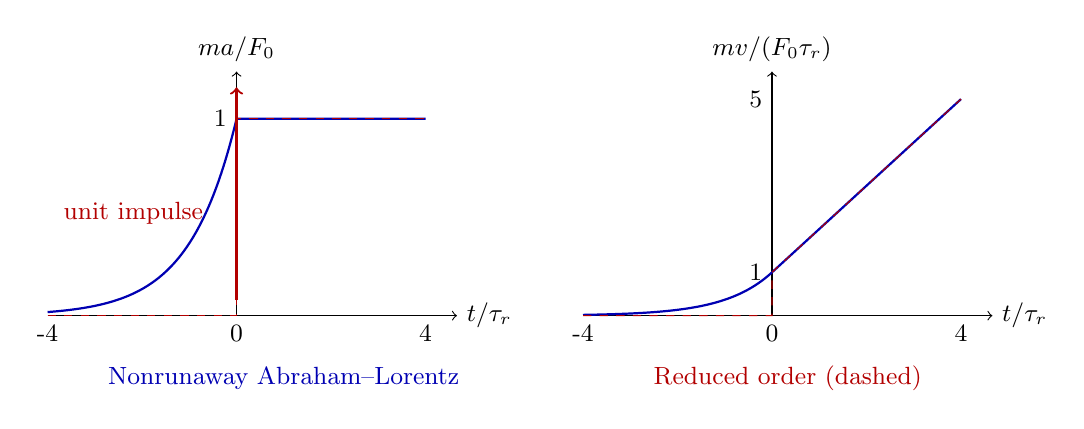
\begin{tikzpicture}[font=\small]
\begin{scope}
\draw[->] (0,0)--(5.2,0) node[right]{$t/\tau_r$};
\draw[->] (2.4,0)--(2.4,3.1) node[above]{$ma/F_0$};
\node[below] at (0.0,0) {-4};
\node[below] at (2.4,0) {0};
\node[below] at (4.8,0) {4};
\node[left] at (2.4,2.5) {$1$};
\draw[blue!70!black,thick] plot coordinates {(0.00000,0.04579) (0.01200,0.04671) (0.02400,0.04766) (0.03600,0.04862) (0.04800,0.04960) (0.06000,0.05060) (0.07200,0.05163) (0.08400,0.05267) (0.09600,0.05373) (0.10800,0.05482) (0.12000,0.05593) (0.13200,0.05706) (0.14400,0.05821) (0.15600,0.05939) (0.16800,0.06058) (0.18000,0.06181) (0.19200,0.06306) (0.20400,0.06433) (0.21600,0.06563) (0.22800,0.06696) (0.24000,0.06831) (0.25200,0.06969) (0.26400,0.07110) (0.27600,0.07253) (0.28800,0.07400) (0.30000,0.07549) (0.31200,0.07702) (0.32400,0.07857) (0.33600,0.08016) (0.34800,0.08178) (0.36000,0.08343) (0.37200,0.08512) (0.38400,0.08684) (0.39600,0.08859) (0.40800,0.09038) (0.42000,0.09221) (0.43200,0.09407) (0.44400,0.09597) (0.45600,0.09791) (0.46800,0.09989) (0.48000,0.10191) (0.49200,0.10396) (0.50400,0.10606) (0.51600,0.10821) (0.52800,0.11039) (0.54000,0.11262) (0.55200,0.11490) (0.56400,0.11722) (0.57600,0.11959) (0.58800,0.12200) (0.60000,0.12447) (0.61200,0.12698) (0.62400,0.12955) (0.63600,0.13216) (0.64800,0.13483) (0.66000,0.13756) (0.67200,0.14034) (0.68400,0.14317) (0.69600,0.14606) (0.70800,0.14901) (0.72000,0.15203) (0.73200,0.15510) (0.74400,0.15823) (0.75600,0.16143) (0.76800,0.16469) (0.78000,0.16801) (0.79200,0.17141) (0.80400,0.17487) (0.81600,0.17840) (0.82800,0.18201) (0.84000,0.18568) (0.85200,0.18944) (0.86400,0.19326) (0.87600,0.19717) (0.88800,0.20115) (0.90000,0.20521) (0.91200,0.20936) (0.92400,0.21359) (0.93600,0.21790) (0.94800,0.22230) (0.96000,0.22679) (0.97200,0.23138) (0.98400,0.23605) (0.99600,0.24082) (1.00800,0.24568) (1.02000,0.25065) (1.03200,0.25571) (1.04400,0.26088) (1.05600,0.26615) (1.06800,0.27152) (1.08000,0.27701) (1.09200,0.28260) (1.10400,0.28831) (1.11600,0.29414) (1.12800,0.30008) (1.14000,0.30614) (1.15200,0.31233) (1.16400,0.31863) (1.17600,0.32507) (1.18800,0.33164) (1.20000,0.33834) (1.21200,0.34517) (1.22400,0.35215) (1.23600,0.35926) (1.24800,0.36652) (1.26000,0.37392) (1.27200,0.38148) (1.28400,0.38918) (1.29600,0.39704) (1.30800,0.40506) (1.32000,0.41325) (1.33200,0.42160) (1.34400,0.43011) (1.35600,0.43880) (1.36800,0.44767) (1.38000,0.45671) (1.39200,0.46593) (1.40400,0.47535) (1.41600,0.48495) (1.42800,0.49475) (1.44000,0.50474) (1.45200,0.51494) (1.46400,0.52534) (1.47600,0.53595) (1.48800,0.54678) (1.50000,0.55783) (1.51200,0.56909) (1.52400,0.58059) (1.53600,0.59232) (1.54800,0.60429) (1.56000,0.61649) (1.57200,0.62895) (1.58400,0.64165) (1.59600,0.65461) (1.60800,0.66784) (1.62000,0.68133) (1.63200,0.69509) (1.64400,0.70914) (1.65600,0.72346) (1.66800,0.73808) (1.68000,0.75299) (1.69200,0.76820) (1.70400,0.78372) (1.71600,0.79955) (1.72800,0.81570) (1.74000,0.83218) (1.75200,0.84899) (1.76400,0.86614) (1.77600,0.88364) (1.78800,0.90149) (1.80000,0.91970) (1.81200,0.93828) (1.82400,0.95723) (1.83600,0.97657) (1.84800,0.99630) (1.86000,1.01642) (1.87200,1.03696) (1.88400,1.05791) (1.89600,1.07928) (1.90800,1.10108) (1.92000,1.12332) (1.93200,1.14602) (1.94400,1.16917) (1.95600,1.19278) (1.96800,1.21688) (1.98000,1.24146) (1.99200,1.26654) (2.00400,1.29213) (2.01600,1.31823) (2.02800,1.34486) (2.04000,1.37203) (2.05200,1.39975) (2.06400,1.42802) (2.07600,1.45687) (2.08800,1.48630) (2.10000,1.51633) (2.11200,1.54696) (2.12400,1.57821) (2.13600,1.61009) (2.14800,1.64262) (2.16000,1.67580) (2.17200,1.70965) (2.18400,1.74419) (2.19600,1.77943) (2.20800,1.81537) (2.22000,1.85205) (2.23200,1.88946) (2.24400,1.92763) (2.25600,1.96657) (2.26800,2.00630) (2.28000,2.04683) (2.29200,2.08818) (2.30400,2.13036) (2.31600,2.17340) (2.32800,2.21730) (2.34000,2.26209) (2.35200,2.30779) (2.36400,2.35441) (2.37600,2.40197) (2.38800,2.45050) (2.40000,2.50000) (2.41200,2.50000) (2.42400,2.50000) (2.43600,2.50000) (2.44800,2.50000) (2.46000,2.50000) (2.47200,2.50000) (2.48400,2.50000) (2.49600,2.50000) (2.50800,2.50000) (2.52000,2.50000) (2.53200,2.50000) (2.54400,2.50000) (2.55600,2.50000) (2.56800,2.50000) (2.58000,2.50000) (2.59200,2.50000) (2.60400,2.50000) (2.61600,2.50000) (2.62800,2.50000) (2.64000,2.50000) (2.65200,2.50000) (2.66400,2.50000) (2.67600,2.50000) (2.68800,2.50000) (2.70000,2.50000) (2.71200,2.50000) (2.72400,2.50000) (2.73600,2.50000) (2.74800,2.50000) (2.76000,2.50000) (2.77200,2.50000) (2.78400,2.50000) (2.79600,2.50000) (2.80800,2.50000) (2.82000,2.50000) (2.83200,2.50000) (2.84400,2.50000) (2.85600,2.50000) (2.86800,2.50000) (2.88000,2.50000) (2.89200,2.50000) (2.90400,2.50000) (2.91600,2.50000) (2.92800,2.50000) (2.94000,2.50000) (2.95200,2.50000) (2.96400,2.50000) (2.97600,2.50000) (2.98800,2.50000) (3.00000,2.50000) (3.01200,2.50000) (3.02400,2.50000) (3.03600,2.50000) (3.04800,2.50000) (3.06000,2.50000) (3.07200,2.50000) (3.08400,2.50000) (3.09600,2.50000) (3.10800,2.50000) (3.12000,2.50000) (3.13200,2.50000) (3.14400,2.50000) (3.15600,2.50000) (3.16800,2.50000) (3.18000,2.50000) (3.19200,2.50000) (3.20400,2.50000) (3.21600,2.50000) (3.22800,2.50000) (3.24000,2.50000) (3.25200,2.50000) (3.26400,2.50000) (3.27600,2.50000) (3.28800,2.50000) (3.30000,2.50000) (3.31200,2.50000) (3.32400,2.50000) (3.33600,2.50000) (3.34800,2.50000) (3.36000,2.50000) (3.37200,2.50000) (3.38400,2.50000) (3.39600,2.50000) (3.40800,2.50000) (3.42000,2.50000) (3.43200,2.50000) (3.44400,2.50000) (3.45600,2.50000) (3.46800,2.50000) (3.48000,2.50000) (3.49200,2.50000) (3.50400,2.50000) (3.51600,2.50000) (3.52800,2.50000) (3.54000,2.50000) (3.55200,2.50000) (3.56400,2.50000) (3.57600,2.50000) (3.58800,2.50000) (3.60000,2.50000) (3.61200,2.50000) (3.62400,2.50000) (3.63600,2.50000) (3.64800,2.50000) (3.66000,2.50000) (3.67200,2.50000) (3.68400,2.50000) (3.69600,2.50000) (3.70800,2.50000) (3.72000,2.50000) (3.73200,2.50000) (3.74400,2.50000) (3.75600,2.50000) (3.76800,2.50000) (3.78000,2.50000) (3.79200,2.50000) (3.80400,2.50000) (3.81600,2.50000) (3.82800,2.50000) (3.84000,2.50000) (3.85200,2.50000) (3.86400,2.50000) (3.87600,2.50000) (3.88800,2.50000) (3.90000,2.50000) (3.91200,2.50000) (3.92400,2.50000) (3.93600,2.50000) (3.94800,2.50000) (3.96000,2.50000) (3.97200,2.50000) (3.98400,2.50000) (3.99600,2.50000) (4.00800,2.50000) (4.02000,2.50000) (4.03200,2.50000) (4.04400,2.50000) (4.05600,2.50000) (4.06800,2.50000) (4.08000,2.50000) (4.09200,2.50000) (4.10400,2.50000) (4.11600,2.50000) (4.12800,2.50000) (4.14000,2.50000) (4.15200,2.50000) (4.16400,2.50000) (4.17600,2.50000) (4.18800,2.50000) (4.20000,2.50000) (4.21200,2.50000) (4.22400,2.50000) (4.23600,2.50000) (4.24800,2.50000) (4.26000,2.50000) (4.27200,2.50000) (4.28400,2.50000) (4.29600,2.50000) (4.30800,2.50000) (4.32000,2.50000) (4.33200,2.50000) (4.34400,2.50000) (4.35600,2.50000) (4.36800,2.50000) (4.38000,2.50000) (4.39200,2.50000) (4.40400,2.50000) (4.41600,2.50000) (4.42800,2.50000) (4.44000,2.50000) (4.45200,2.50000) (4.46400,2.50000) (4.47600,2.50000) (4.48800,2.50000) (4.50000,2.50000) (4.51200,2.50000) (4.52400,2.50000) (4.53600,2.50000) (4.54800,2.50000) (4.56000,2.50000) (4.57200,2.50000) (4.58400,2.50000) (4.59600,2.50000) (4.60800,2.50000) (4.62000,2.50000) (4.63200,2.50000) (4.64400,2.50000) (4.65600,2.50000) (4.66800,2.50000) (4.68000,2.50000) (4.69200,2.50000) (4.70400,2.50000) (4.71600,2.50000) (4.72800,2.50000) (4.74000,2.50000) (4.75200,2.50000) (4.76400,2.50000) (4.77600,2.50000) (4.78800,2.50000) (4.80000,2.50000)};
\draw[red!70!black,dashed] (0,0)--(2.4,0)--(2.4,2.5)--(4.8,2.5);
\draw[red!70!black,->,thick] (2.4,.2)--(2.4,2.9);
\node[red!70!black,anchor=east] at (2.1,1.3) {unit impulse};
\end{scope}
\begin{scope}[xshift=6.8cm]
\draw[->] (0,0)--(5.2,0) node[right]{$t/\tau_r$};
\draw[->] (2.4,0)--(2.4,3.1) node[above]{$mv/(F_0\tau_r)$};
\node[below] at (0.0,0) {-4};
\node[below] at (2.4,0) {0};
\node[below] at (4.8,0) {4};
\draw[blue!70!black,thick] plot coordinates {(0.00000,0.01007) (0.01200,0.01028) (0.02400,0.01048) (0.03600,0.01070) (0.04800,0.01091) (0.06000,0.01113) (0.07200,0.01136) (0.08400,0.01159) (0.09600,0.01182) (0.10800,0.01206) (0.12000,0.01230) (0.13200,0.01255) (0.14400,0.01281) (0.15600,0.01306) (0.16800,0.01333) (0.18000,0.01360) (0.19200,0.01387) (0.20400,0.01415) (0.21600,0.01444) (0.22800,0.01473) (0.24000,0.01503) (0.25200,0.01533) (0.26400,0.01564) (0.27600,0.01596) (0.28800,0.01628) (0.30000,0.01661) (0.31200,0.01694) (0.32400,0.01729) (0.33600,0.01764) (0.34800,0.01799) (0.36000,0.01836) (0.37200,0.01873) (0.38400,0.01910) (0.39600,0.01949) (0.40800,0.01988) (0.42000,0.02029) (0.43200,0.02070) (0.44400,0.02111) (0.45600,0.02154) (0.46800,0.02198) (0.48000,0.02242) (0.49200,0.02287) (0.50400,0.02333) (0.51600,0.02381) (0.52800,0.02429) (0.54000,0.02478) (0.55200,0.02528) (0.56400,0.02579) (0.57600,0.02631) (0.58800,0.02684) (0.60000,0.02738) (0.61200,0.02794) (0.62400,0.02850) (0.63600,0.02908) (0.64800,0.02966) (0.66000,0.03026) (0.67200,0.03087) (0.68400,0.03150) (0.69600,0.03213) (0.70800,0.03278) (0.72000,0.03345) (0.73200,0.03412) (0.74400,0.03481) (0.75600,0.03551) (0.76800,0.03623) (0.78000,0.03696) (0.79200,0.03771) (0.80400,0.03847) (0.81600,0.03925) (0.82800,0.04004) (0.84000,0.04085) (0.85200,0.04168) (0.86400,0.04252) (0.87600,0.04338) (0.88800,0.04425) (0.90000,0.04515) (0.91200,0.04606) (0.92400,0.04699) (0.93600,0.04794) (0.94800,0.04891) (0.96000,0.04989) (0.97200,0.05090) (0.98400,0.05193) (0.99600,0.05298) (1.00800,0.05405) (1.02000,0.05514) (1.03200,0.05626) (1.04400,0.05739) (1.05600,0.05855) (1.06800,0.05974) (1.08000,0.06094) (1.09200,0.06217) (1.10400,0.06343) (1.11600,0.06471) (1.12800,0.06602) (1.14000,0.06735) (1.15200,0.06871) (1.16400,0.07010) (1.17600,0.07152) (1.18800,0.07296) (1.20000,0.07443) (1.21200,0.07594) (1.22400,0.07747) (1.23600,0.07904) (1.24800,0.08063) (1.26000,0.08226) (1.27200,0.08392) (1.28400,0.08562) (1.29600,0.08735) (1.30800,0.08911) (1.32000,0.09091) (1.33200,0.09275) (1.34400,0.09462) (1.35600,0.09654) (1.36800,0.09849) (1.38000,0.10048) (1.39200,0.10251) (1.40400,0.10458) (1.41600,0.10669) (1.42800,0.10884) (1.44000,0.11104) (1.45200,0.11329) (1.46400,0.11557) (1.47600,0.11791) (1.48800,0.12029) (1.50000,0.12272) (1.51200,0.12520) (1.52400,0.12773) (1.53600,0.13031) (1.54800,0.13294) (1.56000,0.13563) (1.57200,0.13837) (1.58400,0.14116) (1.59600,0.14402) (1.60800,0.14692) (1.62000,0.14989) (1.63200,0.15292) (1.64400,0.15601) (1.65600,0.15916) (1.66800,0.16238) (1.68000,0.16566) (1.69200,0.16900) (1.70400,0.17242) (1.71600,0.17590) (1.72800,0.17945) (1.74000,0.18308) (1.75200,0.18678) (1.76400,0.19055) (1.77600,0.19440) (1.78800,0.19833) (1.80000,0.20233) (1.81200,0.20642) (1.82400,0.21059) (1.83600,0.21485) (1.84800,0.21919) (1.86000,0.22361) (1.87200,0.22813) (1.88400,0.23274) (1.89600,0.23744) (1.90800,0.24224) (1.92000,0.24713) (1.93200,0.25212) (1.94400,0.25722) (1.95600,0.26241) (1.96800,0.26771) (1.98000,0.27312) (1.99200,0.27864) (2.00400,0.28427) (2.01600,0.29001) (2.02800,0.29587) (2.04000,0.30185) (2.05200,0.30794) (2.06400,0.31416) (2.07600,0.32051) (2.08800,0.32699) (2.10000,0.33359) (2.11200,0.34033) (2.12400,0.34721) (2.13600,0.35422) (2.14800,0.36138) (2.16000,0.36868) (2.17200,0.37612) (2.18400,0.38372) (2.19600,0.39147) (2.20800,0.39938) (2.22000,0.40745) (2.23200,0.41568) (2.24400,0.42408) (2.25600,0.43265) (2.26800,0.44139) (2.28000,0.45030) (2.29200,0.45940) (2.30400,0.46868) (2.31600,0.47815) (2.32800,0.48781) (2.34000,0.49766) (2.35200,0.50771) (2.36400,0.51797) (2.37600,0.52843) (2.38800,0.53911) (2.40000,0.55000) (2.41200,0.56100) (2.42400,0.57200) (2.43600,0.58300) (2.44800,0.59400) (2.46000,0.60500) (2.47200,0.61600) (2.48400,0.62700) (2.49600,0.63800) (2.50800,0.64900) (2.52000,0.66000) (2.53200,0.67100) (2.54400,0.68200) (2.55600,0.69300) (2.56800,0.70400) (2.58000,0.71500) (2.59200,0.72600) (2.60400,0.73700) (2.61600,0.74800) (2.62800,0.75900) (2.64000,0.77000) (2.65200,0.78100) (2.66400,0.79200) (2.67600,0.80300) (2.68800,0.81400) (2.70000,0.82500) (2.71200,0.83600) (2.72400,0.84700) (2.73600,0.85800) (2.74800,0.86900) (2.76000,0.88000) (2.77200,0.89100) (2.78400,0.90200) (2.79600,0.91300) (2.80800,0.92400) (2.82000,0.93500) (2.83200,0.94600) (2.84400,0.95700) (2.85600,0.96800) (2.86800,0.97900) (2.88000,0.99000) (2.89200,1.00100) (2.90400,1.01200) (2.91600,1.02300) (2.92800,1.03400) (2.94000,1.04500) (2.95200,1.05600) (2.96400,1.06700) (2.97600,1.07800) (2.98800,1.08900) (3.00000,1.10000) (3.01200,1.11100) (3.02400,1.12200) (3.03600,1.13300) (3.04800,1.14400) (3.06000,1.15500) (3.07200,1.16600) (3.08400,1.17700) (3.09600,1.18800) (3.10800,1.19900) (3.12000,1.21000) (3.13200,1.22100) (3.14400,1.23200) (3.15600,1.24300) (3.16800,1.25400) (3.18000,1.26500) (3.19200,1.27600) (3.20400,1.28700) (3.21600,1.29800) (3.22800,1.30900) (3.24000,1.32000) (3.25200,1.33100) (3.26400,1.34200) (3.27600,1.35300) (3.28800,1.36400) (3.30000,1.37500) (3.31200,1.38600) (3.32400,1.39700) (3.33600,1.40800) (3.34800,1.41900) (3.36000,1.43000) (3.37200,1.44100) (3.38400,1.45200) (3.39600,1.46300) (3.40800,1.47400) (3.42000,1.48500) (3.43200,1.49600) (3.44400,1.50700) (3.45600,1.51800) (3.46800,1.52900) (3.48000,1.54000) (3.49200,1.55100) (3.50400,1.56200) (3.51600,1.57300) (3.52800,1.58400) (3.54000,1.59500) (3.55200,1.60600) (3.56400,1.61700) (3.57600,1.62800) (3.58800,1.63900) (3.60000,1.65000) (3.61200,1.66100) (3.62400,1.67200) (3.63600,1.68300) (3.64800,1.69400) (3.66000,1.70500) (3.67200,1.71600) (3.68400,1.72700) (3.69600,1.73800) (3.70800,1.74900) (3.72000,1.76000) (3.73200,1.77100) (3.74400,1.78200) (3.75600,1.79300) (3.76800,1.80400) (3.78000,1.81500) (3.79200,1.82600) (3.80400,1.83700) (3.81600,1.84800) (3.82800,1.85900) (3.84000,1.87000) (3.85200,1.88100) (3.86400,1.89200) (3.87600,1.90300) (3.88800,1.91400) (3.90000,1.92500) (3.91200,1.93600) (3.92400,1.94700) (3.93600,1.95800) (3.94800,1.96900) (3.96000,1.98000) (3.97200,1.99100) (3.98400,2.00200) (3.99600,2.01300) (4.00800,2.02400) (4.02000,2.03500) (4.03200,2.04600) (4.04400,2.05700) (4.05600,2.06800) (4.06800,2.07900) (4.08000,2.09000) (4.09200,2.10100) (4.10400,2.11200) (4.11600,2.12300) (4.12800,2.13400) (4.14000,2.14500) (4.15200,2.15600) (4.16400,2.16700) (4.17600,2.17800) (4.18800,2.18900) (4.20000,2.20000) (4.21200,2.21100) (4.22400,2.22200) (4.23600,2.23300) (4.24800,2.24400) (4.26000,2.25500) (4.27200,2.26600) (4.28400,2.27700) (4.29600,2.28800) (4.30800,2.29900) (4.32000,2.31000) (4.33200,2.32100) (4.34400,2.33200) (4.35600,2.34300) (4.36800,2.35400) (4.38000,2.36500) (4.39200,2.37600) (4.40400,2.38700) (4.41600,2.39800) (4.42800,2.40900) (4.44000,2.42000) (4.45200,2.43100) (4.46400,2.44200) (4.47600,2.45300) (4.48800,2.46400) (4.50000,2.47500) (4.51200,2.48600) (4.52400,2.49700) (4.53600,2.50800) (4.54800,2.51900) (4.56000,2.53000) (4.57200,2.54100) (4.58400,2.55200) (4.59600,2.56300) (4.60800,2.57400) (4.62000,2.58500) (4.63200,2.59600) (4.64400,2.60700) (4.65600,2.61800) (4.66800,2.62900) (4.68000,2.64000) (4.69200,2.65100) (4.70400,2.66200) (4.71600,2.67300) (4.72800,2.68400) (4.74000,2.69500) (4.75200,2.70600) (4.76400,2.71700) (4.77600,2.72800) (4.78800,2.73900) (4.80000,2.75000)};
\draw[red!70!black,dashed] (0,0)--(2.4,0)--(2.4,.55)--(4.8,2.75);
\node[left] at (2.4,.55) {$1$};
\node[left] at (2.4,2.75) {$5$};
\end{scope}
\node[blue!70!black] at (3,-.8) {Nonrunaway Abraham--Lorentz};
\node[red!70!black] at (9.4,-.8) {Reduced order (dashed)};
\end{tikzpicture}
\end{center}

\Needspace{5\baselineskip}
\par\bigskip
\noindent\textbf{16.11}\quad A nonrelativistic particle of charge $e$ and mass $m$ is accelerated in one-dimensional motion across a gap of width $d$ by a constant electric field. The mathematical idealization is that the particle has applied to it an external force $m\alpha$ while its coordinate lies in the interval $(0,d)$. Without radiation damping the particle, having initial velocity $v_{0}$, is accelerated uniformly for a time $T=(-v_{0}/\alpha)+\sqrt{(v_{0}^{2}/\alpha^{2})+(2d/\alpha)}$, emerging at $x=d$ with a final velocity $v_{1}=\sqrt{v_{0}^{2}+2\alpha d}$.

With radiation damping the motion is altered so that the particle takes a time $T'$ to cross the gap and emerges with a velocity $v'_{1}$.
\begin{enumerate}
\item[(a)] Solve the integro-differential equation of motion, including damping, assuming $T$ and $T'$ large compared to $\tau$. Sketch a velocity-versus-time diagram for the motion with and without damping.
\item[(b)] Show that to lowest order in $\tau$,
\begin{align*}
T'&=T-\tau\!\left(1-\frac{v_{0}}{v_{1}}\right)\\[6pt]
v'_{1}&=v_{1}-\frac{\alpha^{2}\tau}{v_{1}}\,T
\end{align*}
\item[(c)] Verify that the sum of the energy radiated and the change in the particle's kinetic energy is equal to the work done by the applied field.
\end{enumerate}
\solution

Let $\tau_r=2e^2/(3mc^3)$, choose entry at $x=0,t=0$, and write
$T'$ for the exit time. The prescribed $v_0$ is the incoming velocity
before the preacceleration region. Take $\alpha>0$, $d>0$, $v_0\ge0$.

\textbf{(a)} Along the monotone crossing trajectory the force is
$m\alpha$ for $0<t<T'$ and zero otherwise. Inserting this finite pulse
in the nonrunaway force integral of 16.10 gives
\[
a(t)=\begin{cases}
\alpha(1-e^{-T'/\tau_r})e^{t/\tau_r},&t<0,\\
\alpha[1-e^{(t-T')/\tau_r}],&0<t<T',\\
0,&t>T'.
\end{cases}
\]
For example in the middle interval the allowed integration range is
$0<s<(T'-t)/\tau_r$, whose exponential integral is
$1-e^{(t-T')/\tau_r}$.
Integrating $a$ and imposing $v(-\infty)=v_0$ gives
\[
\boxed{v(t)=\begin{cases}
v_0+\alpha\tau_r(1-e^{-T'/\tau_r})e^{t/\tau_r},&t<0,\\
v_0+\alpha[t+\tau_r-\tau_r e^{(t-T')/\tau_r}],&0<t<T',\\
v_0+\alpha T',&t>T'.
\end{cases}}
\]
Both transitions are continuous. In particular $v(0)$ is slightly
larger than $v_0$ and $v_1'=v_0+\alpha T'$.
The spatial crossing condition determines $T'$ self-consistently:
\begin{align*}
d=\int_0^{T'}v(t)dt
&=v_0T'+\frac\alpha2T'^2+\alpha\tau_rT'
-\alpha\tau_r^2(1-e^{-T'/\tau_r}).
\end{align*}
Its derivative with respect to $T'$ is
$v_0+\alpha T'+\alpha\tau_r(1-e^{-T'/\tau_r})>0$ for $T'>0$,
so the positive crossing time is unique. For $T'\gg\tau_r$ the
exponential is negligible except in the short entry and exit layers.
The plot compares this solution with the undamped piecewise linear
velocity for one representative $T/\tau_r\gg1$ case.
\begin{center}% Generated by supplementary/check_ch16.py
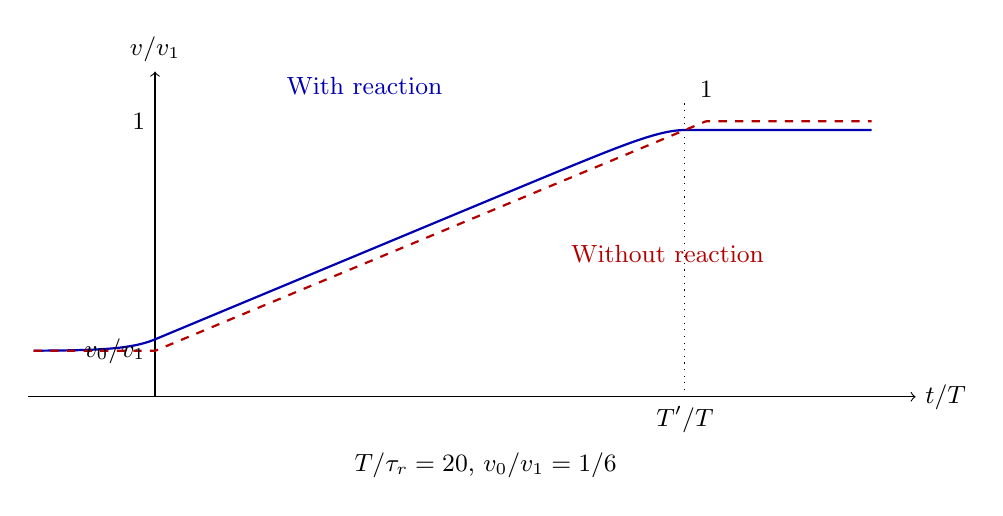
\begin{tikzpicture}[x=7cm,y=3.5cm,font=\small]
\draw[->] (-.23,0)--(1.38,0) node[right]{$t/T$};
\draw[->] (0,0)--(0,1.18) node[above]{$v/v_1$};
\draw[blue!70!black,thick] plot coordinates {(-0.22000,0.16718) (-0.21695,0.16721) (-0.21391,0.16724) (-0.21086,0.16728) (-0.20782,0.16732) (-0.20477,0.16736) (-0.20172,0.16740) (-0.19868,0.16745) (-0.19563,0.16750) (-0.19259,0.16755) (-0.18954,0.16761) (-0.18649,0.16767) (-0.18345,0.16773) (-0.18040,0.16780) (-0.17735,0.16787) (-0.17431,0.16794) (-0.17126,0.16802) (-0.16822,0.16811) (-0.16517,0.16820) (-0.16212,0.16829) (-0.15908,0.16840) (-0.15603,0.16851) (-0.15299,0.16862) (-0.14994,0.16874) (-0.14689,0.16887) (-0.14385,0.16901) (-0.14080,0.16916) (-0.13776,0.16932) (-0.13471,0.16948) (-0.13166,0.16966) (-0.12862,0.16985) (-0.12557,0.17005) (-0.12253,0.17026) (-0.11948,0.17049) (-0.11643,0.17073) (-0.11339,0.17098) (-0.11034,0.17125) (-0.10729,0.17154) (-0.10425,0.17185) (-0.10120,0.17217) (-0.09816,0.17252) (-0.09511,0.17288) (-0.09206,0.17328) (-0.08902,0.17369) (-0.08597,0.17413) (-0.08293,0.17460) (-0.07988,0.17510) (-0.07683,0.17563) (-0.07379,0.17619) (-0.07074,0.17679) (-0.06770,0.17743) (-0.06465,0.17810) (-0.06160,0.17882) (-0.05856,0.17958) (-0.05551,0.18040) (-0.05246,0.18126) (-0.04942,0.18217) (-0.04637,0.18315) (-0.04333,0.18418) (-0.04028,0.18528) (-0.03723,0.18645) (-0.03419,0.18770) (-0.03114,0.18902) (-0.02810,0.19042) (-0.02505,0.19191) (-0.02200,0.19350) (-0.01896,0.19518) (-0.01591,0.19698) (-0.01287,0.19888) (-0.00982,0.20090) (-0.00677,0.20305) (-0.00373,0.20534) (-0.00068,0.20777) (0.00236,0.21030) (0.00541,0.21284) (0.00846,0.21538) (0.01150,0.21792) (0.01455,0.22046) (0.01760,0.22300) (0.02064,0.22553) (0.02369,0.22807) (0.02673,0.23061) (0.02978,0.23315) (0.03283,0.23569) (0.03587,0.23823) (0.03892,0.24076) (0.04196,0.24330) (0.04501,0.24584) (0.04806,0.24838) (0.05110,0.25092) (0.05415,0.25346) (0.05719,0.25600) (0.06024,0.25853) (0.06329,0.26107) (0.06633,0.26361) (0.06938,0.26615) (0.07242,0.26869) (0.07547,0.27123) (0.07852,0.27376) (0.08156,0.27630) (0.08461,0.27884) (0.08766,0.28138) (0.09070,0.28392) (0.09375,0.28646) (0.09679,0.28899) (0.09984,0.29153) (0.10289,0.29407) (0.10593,0.29661) (0.10898,0.29915) (0.11202,0.30169) (0.11507,0.30423) (0.11812,0.30676) (0.12116,0.30930) (0.12421,0.31184) (0.12725,0.31438) (0.13030,0.31692) (0.13335,0.31946) (0.13639,0.32199) (0.13944,0.32453) (0.14248,0.32707) (0.14553,0.32961) (0.14858,0.33215) (0.15162,0.33469) (0.15467,0.33722) (0.15772,0.33976) (0.16076,0.34230) (0.16381,0.34484) (0.16685,0.34738) (0.16990,0.34992) (0.17295,0.35245) (0.17599,0.35499) (0.17904,0.35753) (0.18208,0.36007) (0.18513,0.36261) (0.18818,0.36515) (0.19122,0.36769) (0.19427,0.37022) (0.19731,0.37276) (0.20036,0.37530) (0.20341,0.37784) (0.20645,0.38038) (0.20950,0.38292) (0.21255,0.38545) (0.21559,0.38799) (0.21864,0.39053) (0.22168,0.39307) (0.22473,0.39561) (0.22778,0.39815) (0.23082,0.40068) (0.23387,0.40322) (0.23691,0.40576) (0.23996,0.40830) (0.24301,0.41084) (0.24605,0.41338) (0.24910,0.41592) (0.25214,0.41845) (0.25519,0.42099) (0.25824,0.42353) (0.26128,0.42607) (0.26433,0.42861) (0.26737,0.43115) (0.27042,0.43368) (0.27347,0.43622) (0.27651,0.43876) (0.27956,0.44130) (0.28261,0.44384) (0.28565,0.44638) (0.28870,0.44891) (0.29174,0.45145) (0.29479,0.45399) (0.29784,0.45653) (0.30088,0.45907) (0.30393,0.46161) (0.30697,0.46414) (0.31002,0.46668) (0.31307,0.46922) (0.31611,0.47176) (0.31916,0.47430) (0.32220,0.47684) (0.32525,0.47938) (0.32830,0.48191) (0.33134,0.48445) (0.33439,0.48699) (0.33743,0.48953) (0.34048,0.49207) (0.34353,0.49461) (0.34657,0.49714) (0.34962,0.49968) (0.35267,0.50222) (0.35571,0.50476) (0.35876,0.50730) (0.36180,0.50984) (0.36485,0.51237) (0.36790,0.51491) (0.37094,0.51745) (0.37399,0.51999) (0.37703,0.52253) (0.38008,0.52507) (0.38313,0.52760) (0.38617,0.53014) (0.38922,0.53268) (0.39226,0.53522) (0.39531,0.53776) (0.39836,0.54030) (0.40140,0.54284) (0.40445,0.54537) (0.40749,0.54791) (0.41054,0.55045) (0.41359,0.55299) (0.41663,0.55553) (0.41968,0.55807) (0.42273,0.56060) (0.42577,0.56314) (0.42882,0.56568) (0.43186,0.56822) (0.43491,0.57076) (0.43796,0.57330) (0.44100,0.57583) (0.44405,0.57837) (0.44709,0.58091) (0.45014,0.58345) (0.45319,0.58599) (0.45623,0.58853) (0.45928,0.59106) (0.46232,0.59360) (0.46537,0.59614) (0.46842,0.59868) (0.47146,0.60122) (0.47451,0.60376) (0.47756,0.60629) (0.48060,0.60883) (0.48365,0.61137) (0.48669,0.61391) (0.48974,0.61645) (0.49279,0.61898) (0.49583,0.62152) (0.49888,0.62406) (0.50192,0.62660) (0.50497,0.62914) (0.50802,0.63168) (0.51106,0.63421) (0.51411,0.63675) (0.51715,0.63929) (0.52020,0.64183) (0.52325,0.64437) (0.52629,0.64690) (0.52934,0.64944) (0.53238,0.65198) (0.53543,0.65452) (0.53848,0.65706) (0.54152,0.65959) (0.54457,0.66213) (0.54762,0.66467) (0.55066,0.66721) (0.55371,0.66974) (0.55675,0.67228) (0.55980,0.67482) (0.56285,0.67736) (0.56589,0.67989) (0.56894,0.68243) (0.57198,0.68497) (0.57503,0.68751) (0.57808,0.69004) (0.58112,0.69258) (0.58417,0.69512) (0.58721,0.69766) (0.59026,0.70019) (0.59331,0.70273) (0.59635,0.70527) (0.59940,0.70780) (0.60244,0.71034) (0.60549,0.71288) (0.60854,0.71541) (0.61158,0.71795) (0.61463,0.72048) (0.61768,0.72302) (0.62072,0.72556) (0.62377,0.72809) (0.62681,0.73063) (0.62986,0.73316) (0.63291,0.73570) (0.63595,0.73823) (0.63900,0.74077) (0.64204,0.74330) (0.64509,0.74583) (0.64814,0.74837) (0.65118,0.75090) (0.65423,0.75343) (0.65727,0.75597) (0.66032,0.75850) (0.66337,0.76103) (0.66641,0.76356) (0.66946,0.76609) (0.67251,0.76863) (0.67555,0.77116) (0.67860,0.77369) (0.68164,0.77621) (0.68469,0.77874) (0.68774,0.78127) (0.69078,0.78380) (0.69383,0.78633) (0.69687,0.78885) (0.69992,0.79138) (0.70297,0.79390) (0.70601,0.79642) (0.70906,0.79895) (0.71210,0.80147) (0.71515,0.80399) (0.71820,0.80651) (0.72124,0.80903) (0.72429,0.81154) (0.72733,0.81406) (0.73038,0.81657) (0.73343,0.81909) (0.73647,0.82160) (0.73952,0.82411) (0.74257,0.82661) (0.74561,0.82912) (0.74866,0.83162) (0.75170,0.83412) (0.75475,0.83662) (0.75780,0.83912) (0.76084,0.84161) (0.76389,0.84410) (0.76693,0.84659) (0.76998,0.84908) (0.77303,0.85156) (0.77607,0.85404) (0.77912,0.85651) (0.78216,0.85898) (0.78521,0.86145) (0.78826,0.86391) (0.79130,0.86636) (0.79435,0.86882) (0.79739,0.87126) (0.80044,0.87370) (0.80349,0.87614) (0.80653,0.87856) (0.80958,0.88098) (0.81263,0.88340) (0.81567,0.88580) (0.81872,0.88820) (0.82176,0.89058) (0.82481,0.89296) (0.82786,0.89533) (0.83090,0.89769) (0.83395,0.90003) (0.83699,0.90237) (0.84004,0.90469) (0.84309,0.90700) (0.84613,0.90929) (0.84918,0.91157) (0.85222,0.91383) (0.85527,0.91607) (0.85832,0.91830) (0.86136,0.92050) (0.86441,0.92269) (0.86745,0.92485) (0.87050,0.92699) (0.87355,0.92910) (0.87659,0.93119) (0.87964,0.93325) (0.88269,0.93527) (0.88573,0.93727) (0.88878,0.93923) (0.89182,0.94116) (0.89487,0.94305) (0.89792,0.94489) (0.90096,0.94670) (0.90401,0.94845) (0.90705,0.95016) (0.91010,0.95182) (0.91315,0.95342) (0.91619,0.95496) (0.91924,0.95644) (0.92228,0.95785) (0.92533,0.95919) (0.92838,0.96046) (0.93142,0.96164) (0.93447,0.96274) (0.93752,0.96376) (0.94056,0.96467) (0.94361,0.96548) (0.94665,0.96619) (0.94970,0.96678) (0.95275,0.96725) (0.95579,0.96758) (0.95884,0.96778) (0.96188,0.96784) (0.96493,0.96784) (0.96798,0.96784) (0.97102,0.96784) (0.97407,0.96784) (0.97711,0.96784) (0.98016,0.96784) (0.98321,0.96784) (0.98625,0.96784) (0.98930,0.96784) (0.99234,0.96784) (0.99539,0.96784) (0.99844,0.96784) (1.00148,0.96784) (1.00453,0.96784) (1.00758,0.96784) (1.01062,0.96784) (1.01367,0.96784) (1.01671,0.96784) (1.01976,0.96784) (1.02281,0.96784) (1.02585,0.96784) (1.02890,0.96784) (1.03194,0.96784) (1.03499,0.96784) (1.03804,0.96784) (1.04108,0.96784) (1.04413,0.96784) (1.04717,0.96784) (1.05022,0.96784) (1.05327,0.96784) (1.05631,0.96784) (1.05936,0.96784) (1.06240,0.96784) (1.06545,0.96784) (1.06850,0.96784) (1.07154,0.96784) (1.07459,0.96784) (1.07764,0.96784) (1.08068,0.96784) (1.08373,0.96784) (1.08677,0.96784) (1.08982,0.96784) (1.09287,0.96784) (1.09591,0.96784) (1.09896,0.96784) (1.10200,0.96784) (1.10505,0.96784) (1.10810,0.96784) (1.11114,0.96784) (1.11419,0.96784) (1.11723,0.96784) (1.12028,0.96784) (1.12333,0.96784) (1.12637,0.96784) (1.12942,0.96784) (1.13246,0.96784) (1.13551,0.96784) (1.13856,0.96784) (1.14160,0.96784) (1.14465,0.96784) (1.14770,0.96784) (1.15074,0.96784) (1.15379,0.96784) (1.15683,0.96784) (1.15988,0.96784) (1.16293,0.96784) (1.16597,0.96784) (1.16902,0.96784) (1.17206,0.96784) (1.17511,0.96784) (1.17816,0.96784) (1.18120,0.96784) (1.18425,0.96784) (1.18729,0.96784) (1.19034,0.96784) (1.19339,0.96784) (1.19643,0.96784) (1.19948,0.96784) (1.20253,0.96784) (1.20557,0.96784) (1.20862,0.96784) (1.21166,0.96784) (1.21471,0.96784) (1.21776,0.96784) (1.22080,0.96784) (1.22385,0.96784) (1.22689,0.96784) (1.22994,0.96784) (1.23299,0.96784) (1.23603,0.96784) (1.23908,0.96784) (1.24212,0.96784) (1.24517,0.96784) (1.24822,0.96784) (1.25126,0.96784) (1.25431,0.96784) (1.25735,0.96784) (1.26040,0.96784) (1.26345,0.96784) (1.26649,0.96784) (1.26954,0.96784) (1.27259,0.96784) (1.27563,0.96784) (1.27868,0.96784) (1.28172,0.96784) (1.28477,0.96784) (1.28782,0.96784) (1.29086,0.96784) (1.29391,0.96784) (1.29695,0.96784) (1.30000,0.96784)};
\draw[red!70!black,dashed,thick] plot coordinates {(-0.22000,0.16667) (-0.21695,0.16667) (-0.21391,0.16667) (-0.21086,0.16667) (-0.20782,0.16667) (-0.20477,0.16667) (-0.20172,0.16667) (-0.19868,0.16667) (-0.19563,0.16667) (-0.19259,0.16667) (-0.18954,0.16667) (-0.18649,0.16667) (-0.18345,0.16667) (-0.18040,0.16667) (-0.17735,0.16667) (-0.17431,0.16667) (-0.17126,0.16667) (-0.16822,0.16667) (-0.16517,0.16667) (-0.16212,0.16667) (-0.15908,0.16667) (-0.15603,0.16667) (-0.15299,0.16667) (-0.14994,0.16667) (-0.14689,0.16667) (-0.14385,0.16667) (-0.14080,0.16667) (-0.13776,0.16667) (-0.13471,0.16667) (-0.13166,0.16667) (-0.12862,0.16667) (-0.12557,0.16667) (-0.12253,0.16667) (-0.11948,0.16667) (-0.11643,0.16667) (-0.11339,0.16667) (-0.11034,0.16667) (-0.10729,0.16667) (-0.10425,0.16667) (-0.10120,0.16667) (-0.09816,0.16667) (-0.09511,0.16667) (-0.09206,0.16667) (-0.08902,0.16667) (-0.08597,0.16667) (-0.08293,0.16667) (-0.07988,0.16667) (-0.07683,0.16667) (-0.07379,0.16667) (-0.07074,0.16667) (-0.06770,0.16667) (-0.06465,0.16667) (-0.06160,0.16667) (-0.05856,0.16667) (-0.05551,0.16667) (-0.05246,0.16667) (-0.04942,0.16667) (-0.04637,0.16667) (-0.04333,0.16667) (-0.04028,0.16667) (-0.03723,0.16667) (-0.03419,0.16667) (-0.03114,0.16667) (-0.02810,0.16667) (-0.02505,0.16667) (-0.02200,0.16667) (-0.01896,0.16667) (-0.01591,0.16667) (-0.01287,0.16667) (-0.00982,0.16667) (-0.00677,0.16667) (-0.00373,0.16667) (-0.00068,0.16667) (0.00236,0.16864) (0.00541,0.17118) (0.00846,0.17371) (0.01150,0.17625) (0.01455,0.17879) (0.01760,0.18133) (0.02064,0.18387) (0.02369,0.18641) (0.02673,0.18894) (0.02978,0.19148) (0.03283,0.19402) (0.03587,0.19656) (0.03892,0.19910) (0.04196,0.20164) (0.04501,0.20418) (0.04806,0.20671) (0.05110,0.20925) (0.05415,0.21179) (0.05719,0.21433) (0.06024,0.21687) (0.06329,0.21941) (0.06633,0.22194) (0.06938,0.22448) (0.07242,0.22702) (0.07547,0.22956) (0.07852,0.23210) (0.08156,0.23464) (0.08461,0.23717) (0.08766,0.23971) (0.09070,0.24225) (0.09375,0.24479) (0.09679,0.24733) (0.09984,0.24987) (0.10289,0.25240) (0.10593,0.25494) (0.10898,0.25748) (0.11202,0.26002) (0.11507,0.26256) (0.11812,0.26510) (0.12116,0.26764) (0.12421,0.27017) (0.12725,0.27271) (0.13030,0.27525) (0.13335,0.27779) (0.13639,0.28033) (0.13944,0.28287) (0.14248,0.28540) (0.14553,0.28794) (0.14858,0.29048) (0.15162,0.29302) (0.15467,0.29556) (0.15772,0.29810) (0.16076,0.30063) (0.16381,0.30317) (0.16685,0.30571) (0.16990,0.30825) (0.17295,0.31079) (0.17599,0.31333) (0.17904,0.31587) (0.18208,0.31840) (0.18513,0.32094) (0.18818,0.32348) (0.19122,0.32602) (0.19427,0.32856) (0.19731,0.33110) (0.20036,0.33363) (0.20341,0.33617) (0.20645,0.33871) (0.20950,0.34125) (0.21255,0.34379) (0.21559,0.34633) (0.21864,0.34886) (0.22168,0.35140) (0.22473,0.35394) (0.22778,0.35648) (0.23082,0.35902) (0.23387,0.36156) (0.23691,0.36409) (0.23996,0.36663) (0.24301,0.36917) (0.24605,0.37171) (0.24910,0.37425) (0.25214,0.37679) (0.25519,0.37933) (0.25824,0.38186) (0.26128,0.38440) (0.26433,0.38694) (0.26737,0.38948) (0.27042,0.39202) (0.27347,0.39456) (0.27651,0.39709) (0.27956,0.39963) (0.28261,0.40217) (0.28565,0.40471) (0.28870,0.40725) (0.29174,0.40979) (0.29479,0.41232) (0.29784,0.41486) (0.30088,0.41740) (0.30393,0.41994) (0.30697,0.42248) (0.31002,0.42502) (0.31307,0.42756) (0.31611,0.43009) (0.31916,0.43263) (0.32220,0.43517) (0.32525,0.43771) (0.32830,0.44025) (0.33134,0.44279) (0.33439,0.44532) (0.33743,0.44786) (0.34048,0.45040) (0.34353,0.45294) (0.34657,0.45548) (0.34962,0.45802) (0.35267,0.46055) (0.35571,0.46309) (0.35876,0.46563) (0.36180,0.46817) (0.36485,0.47071) (0.36790,0.47325) (0.37094,0.47578) (0.37399,0.47832) (0.37703,0.48086) (0.38008,0.48340) (0.38313,0.48594) (0.38617,0.48848) (0.38922,0.49102) (0.39226,0.49355) (0.39531,0.49609) (0.39836,0.49863) (0.40140,0.50117) (0.40445,0.50371) (0.40749,0.50625) (0.41054,0.50878) (0.41359,0.51132) (0.41663,0.51386) (0.41968,0.51640) (0.42273,0.51894) (0.42577,0.52148) (0.42882,0.52401) (0.43186,0.52655) (0.43491,0.52909) (0.43796,0.53163) (0.44100,0.53417) (0.44405,0.53671) (0.44709,0.53925) (0.45014,0.54178) (0.45319,0.54432) (0.45623,0.54686) (0.45928,0.54940) (0.46232,0.55194) (0.46537,0.55448) (0.46842,0.55701) (0.47146,0.55955) (0.47451,0.56209) (0.47756,0.56463) (0.48060,0.56717) (0.48365,0.56971) (0.48669,0.57224) (0.48974,0.57478) (0.49279,0.57732) (0.49583,0.57986) (0.49888,0.58240) (0.50192,0.58494) (0.50497,0.58747) (0.50802,0.59001) (0.51106,0.59255) (0.51411,0.59509) (0.51715,0.59763) (0.52020,0.60017) (0.52325,0.60271) (0.52629,0.60524) (0.52934,0.60778) (0.53238,0.61032) (0.53543,0.61286) (0.53848,0.61540) (0.54152,0.61794) (0.54457,0.62047) (0.54762,0.62301) (0.55066,0.62555) (0.55371,0.62809) (0.55675,0.63063) (0.55980,0.63317) (0.56285,0.63570) (0.56589,0.63824) (0.56894,0.64078) (0.57198,0.64332) (0.57503,0.64586) (0.57808,0.64840) (0.58112,0.65094) (0.58417,0.65347) (0.58721,0.65601) (0.59026,0.65855) (0.59331,0.66109) (0.59635,0.66363) (0.59940,0.66617) (0.60244,0.66870) (0.60549,0.67124) (0.60854,0.67378) (0.61158,0.67632) (0.61463,0.67886) (0.61768,0.68140) (0.62072,0.68393) (0.62377,0.68647) (0.62681,0.68901) (0.62986,0.69155) (0.63291,0.69409) (0.63595,0.69663) (0.63900,0.69916) (0.64204,0.70170) (0.64509,0.70424) (0.64814,0.70678) (0.65118,0.70932) (0.65423,0.71186) (0.65727,0.71440) (0.66032,0.71693) (0.66337,0.71947) (0.66641,0.72201) (0.66946,0.72455) (0.67251,0.72709) (0.67555,0.72963) (0.67860,0.73216) (0.68164,0.73470) (0.68469,0.73724) (0.68774,0.73978) (0.69078,0.74232) (0.69383,0.74486) (0.69687,0.74739) (0.69992,0.74993) (0.70297,0.75247) (0.70601,0.75501) (0.70906,0.75755) (0.71210,0.76009) (0.71515,0.76263) (0.71820,0.76516) (0.72124,0.76770) (0.72429,0.77024) (0.72733,0.77278) (0.73038,0.77532) (0.73343,0.77786) (0.73647,0.78039) (0.73952,0.78293) (0.74257,0.78547) (0.74561,0.78801) (0.74866,0.79055) (0.75170,0.79309) (0.75475,0.79562) (0.75780,0.79816) (0.76084,0.80070) (0.76389,0.80324) (0.76693,0.80578) (0.76998,0.80832) (0.77303,0.81086) (0.77607,0.81339) (0.77912,0.81593) (0.78216,0.81847) (0.78521,0.82101) (0.78826,0.82355) (0.79130,0.82609) (0.79435,0.82862) (0.79739,0.83116) (0.80044,0.83370) (0.80349,0.83624) (0.80653,0.83878) (0.80958,0.84132) (0.81263,0.84385) (0.81567,0.84639) (0.81872,0.84893) (0.82176,0.85147) (0.82481,0.85401) (0.82786,0.85655) (0.83090,0.85908) (0.83395,0.86162) (0.83699,0.86416) (0.84004,0.86670) (0.84309,0.86924) (0.84613,0.87178) (0.84918,0.87432) (0.85222,0.87685) (0.85527,0.87939) (0.85832,0.88193) (0.86136,0.88447) (0.86441,0.88701) (0.86745,0.88955) (0.87050,0.89208) (0.87355,0.89462) (0.87659,0.89716) (0.87964,0.89970) (0.88269,0.90224) (0.88573,0.90478) (0.88878,0.90731) (0.89182,0.90985) (0.89487,0.91239) (0.89792,0.91493) (0.90096,0.91747) (0.90401,0.92001) (0.90705,0.92255) (0.91010,0.92508) (0.91315,0.92762) (0.91619,0.93016) (0.91924,0.93270) (0.92228,0.93524) (0.92533,0.93778) (0.92838,0.94031) (0.93142,0.94285) (0.93447,0.94539) (0.93752,0.94793) (0.94056,0.95047) (0.94361,0.95301) (0.94665,0.95554) (0.94970,0.95808) (0.95275,0.96062) (0.95579,0.96316) (0.95884,0.96570) (0.96188,0.96824) (0.96493,0.97077) (0.96798,0.97331) (0.97102,0.97585) (0.97407,0.97839) (0.97711,0.98093) (0.98016,0.98347) (0.98321,0.98601) (0.98625,0.98854) (0.98930,0.99108) (0.99234,0.99362) (0.99539,0.99616) (0.99844,0.99870) (1.00148,1.00000) (1.00453,1.00000) (1.00758,1.00000) (1.01062,1.00000) (1.01367,1.00000) (1.01671,1.00000) (1.01976,1.00000) (1.02281,1.00000) (1.02585,1.00000) (1.02890,1.00000) (1.03194,1.00000) (1.03499,1.00000) (1.03804,1.00000) (1.04108,1.00000) (1.04413,1.00000) (1.04717,1.00000) (1.05022,1.00000) (1.05327,1.00000) (1.05631,1.00000) (1.05936,1.00000) (1.06240,1.00000) (1.06545,1.00000) (1.06850,1.00000) (1.07154,1.00000) (1.07459,1.00000) (1.07764,1.00000) (1.08068,1.00000) (1.08373,1.00000) (1.08677,1.00000) (1.08982,1.00000) (1.09287,1.00000) (1.09591,1.00000) (1.09896,1.00000) (1.10200,1.00000) (1.10505,1.00000) (1.10810,1.00000) (1.11114,1.00000) (1.11419,1.00000) (1.11723,1.00000) (1.12028,1.00000) (1.12333,1.00000) (1.12637,1.00000) (1.12942,1.00000) (1.13246,1.00000) (1.13551,1.00000) (1.13856,1.00000) (1.14160,1.00000) (1.14465,1.00000) (1.14770,1.00000) (1.15074,1.00000) (1.15379,1.00000) (1.15683,1.00000) (1.15988,1.00000) (1.16293,1.00000) (1.16597,1.00000) (1.16902,1.00000) (1.17206,1.00000) (1.17511,1.00000) (1.17816,1.00000) (1.18120,1.00000) (1.18425,1.00000) (1.18729,1.00000) (1.19034,1.00000) (1.19339,1.00000) (1.19643,1.00000) (1.19948,1.00000) (1.20253,1.00000) (1.20557,1.00000) (1.20862,1.00000) (1.21166,1.00000) (1.21471,1.00000) (1.21776,1.00000) (1.22080,1.00000) (1.22385,1.00000) (1.22689,1.00000) (1.22994,1.00000) (1.23299,1.00000) (1.23603,1.00000) (1.23908,1.00000) (1.24212,1.00000) (1.24517,1.00000) (1.24822,1.00000) (1.25126,1.00000) (1.25431,1.00000) (1.25735,1.00000) (1.26040,1.00000) (1.26345,1.00000) (1.26649,1.00000) (1.26954,1.00000) (1.27259,1.00000) (1.27563,1.00000) (1.27868,1.00000) (1.28172,1.00000) (1.28477,1.00000) (1.28782,1.00000) (1.29086,1.00000) (1.29391,1.00000) (1.29695,1.00000) (1.30000,1.00000)};
\draw[dotted] (0.9614041439493674,0)--(0.9614041439493674,1.08);
\node[below] at (0.9614041439493674,0) {$T^\prime/T$};
\node[above] at (1,1.05) {$1$};
\node[left] at (0,.166667) {$v_0/v_1$};
\node[left] at (0,1) {$1$};
\node[blue!70!black] at (.38,1.13) {With reaction};
\node[red!70!black] at (.93,.52) {Without reaction};
\node at (.6,-.25) {$T/\tau_r=20$, $v_0/v_1=1/6$};
\end{tikzpicture}
\end{center}

\textbf{(b)} Write $T'=T+\delta T$ in the crossing condition and use
$d=v_0T+\alpha T^2/2$. Keeping terms linear in $\tau_r$ gives
\[
0=(v_0+\alpha T)\delta T+\alpha\tau_rT+O(\tau_r^2),\qquad
\delta T=-\frac{\alpha\tau_rT}{v_1},\quad v_1=v_0+\alpha T.
\]
Therefore
\[
\boxed{T'=T-\tau_r(1-v_0/v_1)+O(\tau_r^2),\qquad
v_1'=v_1-\frac{\alpha^2\tau_rT}{v_1}+O(\tau_r^2).}
\]
The earlier entry preacceleration shortens the time spent in the gap,
while the final kinetic energy is lower because energy is radiated.

\textbf{(c)} With $E=e^{-T'/\tau_r}$, integrate the squared acceleration
on the two nonzero intervals:
\[
\int_{-\infty}^0a^2dt=\frac{\alpha^2\tau_r}{2}(1-E)^2,
\quad
\int_0^{T'}a^2dt=\alpha^2
\left[T'-2\tau_r(1-E)+\frac{\tau_r}{2}(1-E^2)\right].
\]
Their sum is $\alpha^2[T'-\tau_r(1-E)]$.
Since the Larmor power is $m\tau_ra^2$,
\[
W_{\rm rad}=m\tau_r\alpha^2[T'-\tau_r(1-E)],\qquad
\Delta K=m\alpha(v_0T'+\alpha T'^2/2).
\]
Adding and using the exact crossing condition gives
\[
\boxed{\Delta K+W_{\rm rad}=m\alpha d=W_{\rm ext}.}
\]
This equality includes the radiation before entry. In the local
Abraham--Lorentz energy equation the extra total derivative is the
Schott term $m\tau_rva$; it vanishes at both asymptotic endpoints,
which is why it does not alter the integrated balance.

\Needspace{5\baselineskip}
\par\bigskip
\noindent\textbf{16.12}\quad A classical model for the description of collision broadening of spectral lines is that the oscillator is interrupted by a collision after oscillating for a time $T$ so that the coherence of the wave train is lost.
\begin{enumerate}
\item[(a)] Taking the oscillator used in Section 16.7 and assuming that the probability that a collision will occur between time $T$ and $(T+dT)$ is $(\nu e^{-\nu T}\;dT)$, where $\nu$ is the mean collision frequency, show that the averaged spectral distribution is
\[
\frac{dI(\omega)}{d\omega}=\frac{I_{0}}{2\pi}\frac{\Gamma+2\nu}{(\omega-\omega_{0})^{2}+\left(\dfrac{\Gamma}{2}+\nu\right)^{2}}
\]
so that the breadth of the line is $(2\nu+\Gamma)$.
\item[(b)] For the sodium doublet at 5893 \AA\ the oscillator strength is $f=0.975$, so that the natural width is essentially the classical value, $\Delta\lambda=1.2\times10^{-4}$ \AA. Estimate the Doppler width of the line, assuming the sodium atoms are in thermal equilibrium at a temperature of 500K, and compare it with the natural width. Assuming a collision cross section of $10^{-16}$ cm$^{2}$, determine the collision breadth of the sodium doublet as a function of the pressure of the sodium vapor. For what pressure is the collision breadth equal to the natural breadth? The Doppler breadth?
\end{enumerate}
\solution

\textbf{(a)} Treat a collision as destroying phase coherence, with
uncorrelated phases after it, while retaining the specified radiative
amplitude decay $e^{-\Gamma t/2}$. This is the phase-interruption model
in the question. Let $I_0$ be the total radiated energy, as in (16.72),
and put $\Delta=\omega-\omega_0$, absorbing any small fixed line shift
in $\omega_0$.
For two times separated by $s$, the probability of no intervening
collision is obtained directly from the given waiting-time density:
\[
\Pr(T>s)=\int_s^\infty\nu e^{-\nu T}dT=e^{-\nu s}.
\]
Products of amplitudes before and after an intervening collision average
to zero. Thus the averaged squared Fourier amplitude is proportional to
\begin{align*}
\mathcal S(\Delta)
&=\int_0^\infty dt\int_0^\infty dt'\,
 e^{-\Gamma(t+t')/2}e^{-\nu|t-t'|}e^{i\Delta(t-t')}\\
&=2\operatorname{Re}\int_0^\infty du\,e^{-\Gamma u}
 \int_0^\infty ds\,e^{-(\Gamma/2+\nu-i\Delta)s}\\
&=\frac2\Gamma\operatorname{Re}\frac1{\Gamma/2+\nu-i\Delta}
=\frac{\Gamma+2\nu}{\Gamma[\Delta^2+(\Gamma/2+\nu)^2]}.
\end{align*}
Here the two triangles $t>t'$ and $t<t'$ use $u=\min(t,t')$ and
$s=|t-t'|$; their diagonal has zero integration measure.
The same normalization as the uncollided wave train is
$I_0\Gamma/(2\pi)$, giving
\[
\boxed{\frac{dI}{d\omega}=\frac{I_0}{2\pi}
\frac{\Gamma+2\nu}{(\omega-\omega_0)^2+(\Gamma/2+\nu)^2}.}
\]
Its area over the narrow-line frequency approximation is $I_0$.
At half maximum $|\Delta|=\Gamma/2+\nu$, so the full width at half
maximum is $\Gamma+2\nu$.
Permanently terminating radiation at the first collision would also
reduce the total energy; it is not the phase-loss model just averaged.

\textbf{(b)} Use full widths at half maximum throughout, consistent
with the line-breadth convention of Section 16.7.
The line-of-sight Maxwell distribution is proportional to
$e^{-Mv_z^2/(2k_BT)}$. With $\delta\omega=\omega_0v_z/c$,
its half-maximum points obey
$Mv_z^2/(2k_BT)=\ln2$. Thus
\[
\Delta\lambda_D=\lambda_0\sqrt{\frac{8k_BT\ln2}{Mc^2}}.
\]
For $M\simeq23\,u$, $T=500$ K, and $\lambda_0=5893$ \AA,
\[
\boxed{\Delta\lambda_D=1.96794\times10^{-2}\ \text{\AA},}
\]
about $164$ times the supplied natural width
$\Delta\lambda_{\!N}=1.2\times10^{-4}$ \AA.
The one-sided $1/e$ Gaussian width is smaller by $2\sqrt{\ln2}$;
it must not be compared as if it were the full width.

For collisions of identical sodium atoms, the relative Maxwell speed
has reduced mass $M/2$, and its mean is
$\bar v_{\rm rel}=\sqrt{16k_BT/(\pi M)}=959.45$ m/s.
Using ideal-gas density $n=P/(k_BT)$ and the given
$\sigma=10^{-16}$ cm$^2=10^{-20}$ m$^2$,
\[
\nu=n\sigma\bar v_{\rm rel}
=(1.38986\times10^3\ {\rm s}^{-1}{\rm Pa}^{-1})P.
\]
The collision contribution to angular-frequency FWHM is $2\nu$.
Since $|d\lambda/d\omega|=\lambda_0^2/(2\pi c)$,
\[
\boxed{\Delta\lambda_C=\frac{\lambda_0^2\nu}{\pi c}
=(5.12474\times10^{-9}\ \text{\AA/Pa})P
=(6.83243\times10^{-7}\ \text{\AA/Torr})P_{\rm Torr}.}
\]
Consequently
\[
\boxed{P_{C=N}=2.34158\times10^4\ {\rm Pa}\simeq176\ {\rm Torr},}
\qquad
\boxed{P_{C=D}=3.84007\times10^6\ {\rm Pa}\simeq28{,}800\ {\rm Torr}.}
\]
These are estimates within the specified constant-cross-section,
ideal-gas collision model. The comparisons are between individual
broadening contributions; a Gaussian Doppler profile convolved with
a Lorentzian natural/collision profile is a Voigt profile, whose total
width is not obtained by simply adding all three widths.

\Needspace{5\baselineskip}
\par\bigskip
\noindent\textbf{16.13}\quad A single particle oscillator under the action of an applied electric field $\mathbf{E}_{0}e^{-i\omega t}$ has a dipole moment given by
\[
\mathbf{p}=\alpha(\omega)\mathbf{E}_{0}e^{-i\omega t}
\]
\begin{enumerate}
\item[(a)] Show that the total dipole cross section can be written as
\[
\sigma_{t}(\omega)=\frac{2\pi}{c}\,[-i\omega\alpha(\omega)+\text{c.c.}]
\]
\item[(b)] Using only the facts that all the normal modes of oscillation must have some damping and that the polarizability $\alpha(\omega)$ must approach the free-particle value $(-e^{2}/m\omega^{2})$ at high frequencies, show that the cross section satisfies the dipole sum rule,
\[
\int_{0}^{\infty}\sigma_{t}(\omega)\;d\omega=\frac{2\pi^{2}e^{2}}{mc}
\]
(The discussion of Kramers--Kronig dispersion relations in Chapter 7 is clearly relevant.)
\end{enumerate}
\solution

\textbf{(a)} The total cross section means extinction, namely scattering
plus any absorption. For phasor $\mathbf p=\alpha\mathbf E_0$,
the mean work taken from the incident field is
\[
\overline P=\frac12\operatorname{Re}
[(-i\omega\mathbf p)\cdot\mathbf E_0^*]
=\frac\omega2\operatorname{Im}\alpha\,|\mathbf E_0|^2.
\]
The incident plane-wave flux in Gaussian units is
$c|\mathbf E_0|^2/(8\pi)$. Dividing gives
\[
\boxed{\sigma_t=\frac{4\pi\omega}{c}\operatorname{Im}\alpha
=\frac{2\pi}{c}[-i\omega\alpha+\text{c.c.}].}
\]
If the only damping is radiative this equals the total scattered power
cross section; otherwise it also contains the absorbed part.

\textbf{(b)} The causal response of a stable damped oscillator is
analytic for $\operatorname{Im}z>0$; its normal-mode poles lie below
the real axis. A real time-domain response also gives
$\alpha(-\omega)=\alpha(\omega)^*$.
Consider $z\alpha(z)$ on a semicircle of radius $R$ in the upper
half-plane, traversed counterclockwise, with the real segment going
from $-R$ to $R$. The specified high-frequency limit is
$z\alpha(z)\sim-e^2/(mz)$.
On the arc $z=Re^{i\theta}$, $dz=iz\,d\theta$, hence
\[
\lim_{R\to\infty}\int_{\rm arc}z\alpha(z)dz
=-\frac{ie^2}{m}\int_0^\pi d\theta=-\frac{i\pi e^2}{m}.
\]
There are no enclosed poles, so the real-axis integral is
$i\pi e^2/m$. Pair its negative and positive parts using the reality
relation:
\[
\int_{-\infty}^{\infty}\omega\alpha(\omega)d\omega
=\int_0^\infty\omega[\alpha(\omega)-\alpha(\omega)^*]d\omega
=2i\int_0^\infty\omega\operatorname{Im}\alpha(\omega)d\omega.
\]
It follows that $\int_0^\infty\omega\operatorname{Im}\alpha\,d\omega
=\pi e^2/(2m)$. Multiplication by the factor in (a) proves
\[
\boxed{\int_0^\infty\sigma_t(\omega)d\omega
=\frac{2\pi^2e^2}{mc}.}
\]
The sum does not depend on the resonance frequencies or widths.
The analyticity and high-frequency behavior are essential: extending
a low-frequency radiation-reaction approximation beyond its validity
can introduce an upper-half-plane runaway pole or the wrong asymptotic
mass, in which case that approximate response cannot be used for this
contour proof.
